%!TEX root = these.tex

\chapter[État de l'art des techniques de sélection]{État de l'art des techniques de sélection}
\minitoc
\label{chap2}
\cleardoublepage

\section{Introduction}
	\subsection{Pointage, sélection et loi de Fitts}
	Le pointage et la sélection de cibles sont de vieux problèmes. Si les cas qui nous intéressent, énumérés dans le chapitre précédent, présentent des difficultés particulières, de nombreuses techniques existent déjà et certaines d'entre elles tiennent compte d'une partie de ces difficultés. L'on peut faire remonter l'histoire de la recherche sur le pointage au moins jusqu'à la loi de Fitts~\cite{fitts1954information}. Celle-ci fut établie notamment grâce à une expérience simple, dans laquelle on demandait aux sujets de toucher certaines zones à l'aide d'un stylet, comme illustré par la figure~\ref{fig:fitts}, et détaillé par sa légende.
	
	\begin{figure}[H]
		\centering
		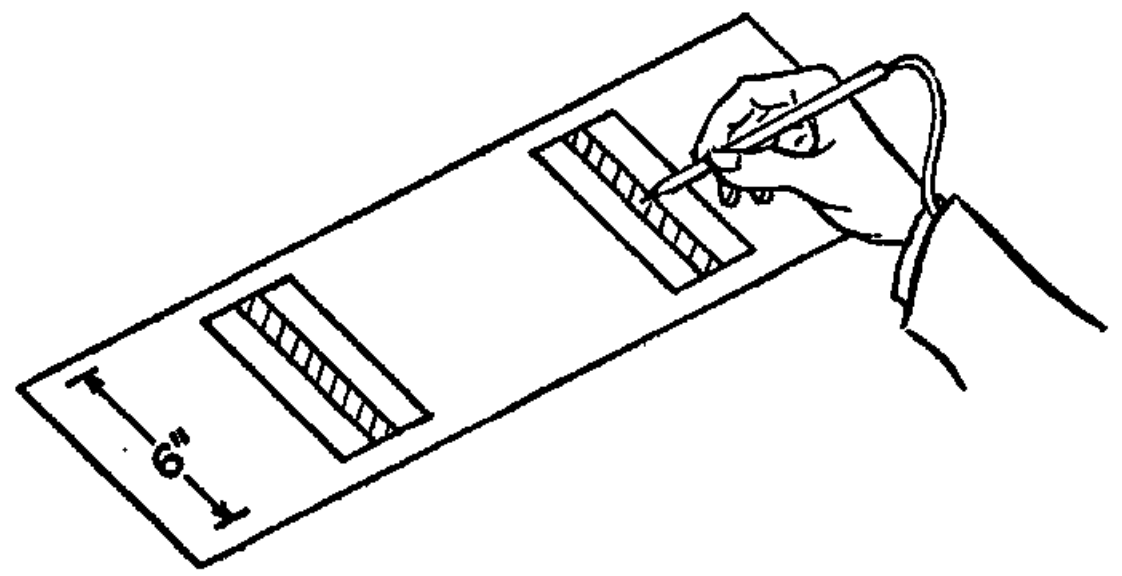
\includegraphics[width=\textwidth]{figures/ch2/fitts}
		\caption[Expérience de Paul M. Fitts.]{Illustration de la première expérience ayant mené Paul Fitts a la découverte de sa loi. Deux triplets de plaques étaient séparés d'une certaine distance. Les sujets devaient, avec leur stylet \og tapoter \fg{} alternativement les deux plaques centrales de chaque triplet, hachurées sur ce schéma, sans toucher les plaques adjacentes. On pouvait faire varier la largeur des plaques ciblées, ainsi que la distance entre elles. Crédit : Paul M. Fitts~\cite{fitts1954information}.}
		\label{fig:fitts}
	\end{figure}
	
	Paul M. Fitts a donc pu déduire de cette étude la loi qui porte son nom, et que l'on peut décrire par les équations~\ref{eq:fitts} et~\ref{eq:fittsID}.
	
	\begin{equation}
		\label{eq:fitts}
		MT = a + bID
	\end{equation}
	
	\begin{equation}
		\label{eq:fittsID}
		ID = \log_2\left(\frac{2D}{W} \right)
	\end{equation}
	
	Dans l'équation~\ref{eq:fitts}, $MT$ représente le temps de mouvement, $a$ et $b$ sont des constantes déterminées empiriquement. Dans l'équation~\ref{eq:fittsID}, $ID$ représente l'indice de difficulté, $D$ représente l'amplitude du mouvement, c'est-à-dire la distance entre la cible et le point de départ du mouvement, tandis que $W$ représente la largeur de la cible. La partie la plus intéressante de cette équation est l'indice de difficulté. C'est la seule partie variable, et c'est celle qui, comme son nom l'indique, détermine la difficulté de la tâche. Cet indice est aisé à comprendre intuitivement : plus l'amplitude du mouvement nécessaire est grande, plus la tâche sera difficile ; plus la largeur de la cible est grande, plus la tâche sera facile.
	
	Pour l'indice de difficulté, MacKenzie propose une formulation de l'indice de difficulté dite de Shannon, inspirée de la théorie de l'information proposée par ce dernier~\cite{mackenzie1989note}. Cette formulation est fournie dans l'équation~\ref{eq:shannon}.
	
	\begin{equation}
		\label{eq:shannon}
		ID = \log_2\left(\frac{D}{W} + 1\right)
	\end{equation}
	
	\subsection{Extensions de la loi de Fitts}
	L'étude de Paul M. Fitts portait sur un dispositif mécanique simple, mais sa loi s'applique aussi bien aux périphériques de saisie classiques (souris, \emph{joysticks}, etc.)~\cite{card1978evaluation}. Mieux, alors qu'elle fut d'abord énoncée pour des mouvements sur une seule dimension, elle loi s'étend aisément au plan~\cite{card1978evaluation, mackenzie1992extending}, éventuellement en tenant compte de la forme de la cible~\cite{accot2003refining}, ou même à l'espace tridimensionnel~\cite{murata2001extending}. On peut également généraliser la loi de Fitts pour modéliser des tâches de tracé de trajectoires~\cite{accot1997beyond, accot1999performance}.
	
	Bien que la loi de Fitts soit d'une élégante simplicité et d'une utilité évidente pour modéliser les performances de sélection, de nombreuses formulations plus ou moins différentes existent, et leurs mérites respectifs font débat~\cite{casallas2015prediction}. Certaines formulations peuvent, par exemple, tenir compte de l'angle $\theta$ entre le vecteur qui va du curseur à la cible et un vecteur horizontal orienté vers la droite (cf. la figure~\ref{fig:theta}). C'est le cas de la formulation de~\cite{murata2001extending} exposée dans l'équation~\ref{eq:murata}.
	
	\begin{equation}
		\label{eq:murata}
		ID = \log_2\left(\frac{D}{W} + 1\right) + c \sin \theta
	\end{equation}
	
	\begin{figure}[ht]
		\centering
		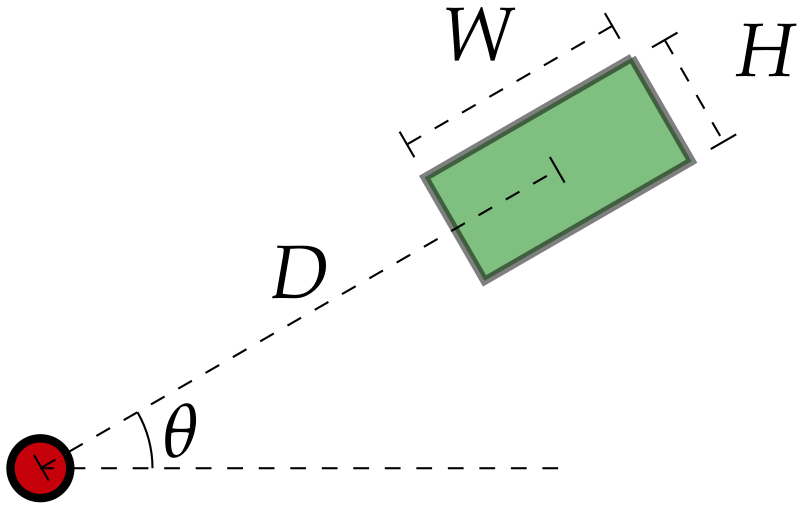
\includegraphics[width=\textwidth]{figures/ch2/theta}
		\caption[Fitts et $\theta$]{Angle $\theta$ pris en compte par~\cite{murata2001extending} dans une version étendue de la loi de Fitts, présentée dans l'équation~\ref{eq:murata}. Le disque rouge représente le curseur, tandis que le rectangle vert représente la cible, située à une distance $D$ du curseur, avec sa largeur $W$ et sa hauteur $H$. Crédit : \cite{casallas2015prediction}.}
		\label{fig:theta}
	\end{figure}
	
	D'autres versions tiennent compte simultanément de la forme de la cible et de cet angle $\theta$~\cite{appert2008evaluation, grossman2004pointing}.
	
	\subsection{Loi de Fitts et cibles mobiles}
	La recherche sur la loi de Fitts appliquée aux cibles mobiles, comparativement aux travaux sur les cibles statiques, est très pauvre~\cite{casallas2015prediction}. Elle n'est pas inexistante~\cite{jagacinski1980test, hoffmann1991capture, hajri2011moving} mais très limitée, et elle s'intéresse rarement à la nature du mouvement des cibles, surtout quand ce mouvement est imprévisible.
	
	De fait, les modèles développés dans les travaux de Jagacinski \emph{et al.}~\cite{jagacinski1980test} ou d'Al Harji \emph{et al.}~\cite{hajri2011moving}, par exemple, font l'hypothèse de cibles de vitesse et de direction constantes. La loi de Fitts étendue par Jagacinski \emph{et al.} est présentée dans l'équation~\ref{eq:jagacinski}, où $CT$ est le temps de sélection, $D$ et $W$ sont toujours la distance à la cible et sa largeur, $V$ est la vitesse de la cible, tandis que $c$, $d$ et $e$ sont des constantes réelles.
	
	\begin{equation}
		\label{eq:jagacinski}
		CT = c + dD + e(V + 1) \left(\frac{1}{W} - 1\right)
	\end{equation}
	
	Les travaux d'Al Harji \emph{et al.}~\cite{hajri2011moving} vont plus loin en tenant compte de la direction de la cible. Les auteurs ont développé deux modèles basés sur ce principe. Le premier est défini par l'équation~\ref{eq:hajriC2}, où $\vec{F}$ est un vecteur déterminé empiriquement, $\vec{D}$ est le vecteur distance entre le curseur et la cible, $\vec{V}$ est le vecteur de vélocité de la cible, et $\vec{R} = \frac{1}{2} \begin{pmatrix}
	W \\ H \\
	\end{pmatrix}$.
	
	Le second est défini par l'équation~\ref{eq:hajriVW}, où $f_{W'}(\theta)$ est un paramètre empirique dépendant de $\theta$, l'angle formé par la direction du mouvement de la cible et l'horizontale. De même $K$ est un paramètre empirique. $D$ est la distance entre le curseur et la cible, $V$ est la vitesse de la cible, et $W'$ est sa largeur dans la direction du mouvement.
	
	\begin{equation}
		\label{eq:hajriC2}
		ID_{C2} = \log_{2}\left(\abs*{\vec{F} \frac{\vec{D}+\vec{V}}{\vec{R}-\vec{V}}} + 1 \right)
	\end{equation}
	
	\begin{equation}
		\label{eq:hajriVW}
		ID_{VWtW'\theta} = \log_{2}\left( f_{W'}(\theta) \left( \frac{D \pm \frac{V}{K}}{\frac{W'}{2} - \frac{V}{K}} \right) \right)
	\end{equation}
	
	Les corrélations entre ces indices de difficulté et les temps de sélection mesurés par Al Hajri \emph{et al.} sont présentées sur la figure~\ref{fig:holdID}, où l'on observera qu'elles sont très fortes. Néanmoins, ces travaux ne portent que sur des cibles dont la vitesse et la direction sont constantes.
	
	\begin{figure}[H]
		\centering
		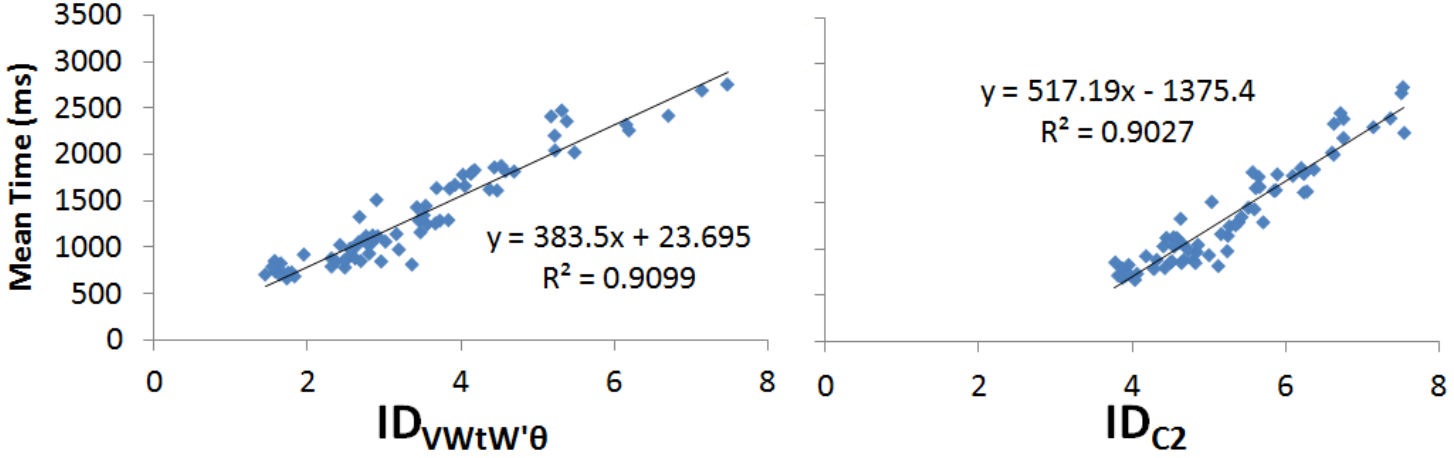
\includegraphics[width=\textwidth]{figures/ch2/holdID}
		\caption[Indice de difficulté en fonction de la nature du mouvement et temps de sélection]{Temps de sélection en fonction des indices de difficulté développés par Al Harji \emph{et al.} Les deux indices sont très fortement corrélés avec les temps de sélection mesurés (sans aucune assistance à la sélection). Crédit : \cite{hajri2011moving}.}
		\label{fig:holdID}
	\end{figure}
	
	D'autres travaux s'attachent à développer des techniques de sélection de cibles mobiles « quelconques » --- c'est-à-dire de direction et de vitesse potentiellement changeantes --- sans nécessairement s'attarder sur les aspects théoriques~\cite{hasan2011comet, ortega2013hook}, et donc sans chercher à étendre la loi de Fitts.
	
	Celle-ci demeure donc, à notre connaissance, incapable de modéliser la difficulté de sélection de cibles mobiles dont la direction peut changer de façon aléatoire, ce qui la rend d'une utilité discutable pour certaines des applications identifiées plus haut, et particulièrement pour les simulations moléculaires interactives, caractérisées par l'imprévisibilité des mouvements de leurs cibles.

\section{Curseurs zonaux}
	\subsection{Principe et avantages généraux}
	Un curseur zonal substitue au curseur ordinaire, qui est réduit à un point, une zone de sélection~\cite{kabbash1995prince, worden1997making}. Lorsque la cible est petite, les performances de sélection ne sont donc plus limitées par sa taille, mais par la taille du curseur. De plus, la distance effective entre le curseur et la cible est légèrement réduite, puisqu'il faut la mesurer à partir de la limite de la zone de sélection, et non depuis son centre.
	
	\subsection{\emph{Prince}}
	La technique \emph{Prince}~\cite{kabbash1995prince} consiste à utiliser un rectangle comme curseur de sélection. Les auteurs ont notamment répliqué la fameuse expérience de Fitts en l'inversant : au lieu d'un point comme curseur et de cibles « larges », ils optèrent pour un curseur large et des cibles ponctuelles, comme l'illustre la figure~\ref{fig:princeCursor}.
	
	\begin{figure}[ht]
		\centering
		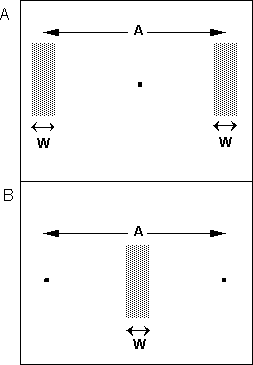
\includegraphics[width=\textwidth]{figures/ch2/princeCursor}
		\caption[\emph{Prince} et son curseur]{En haut, une représentation schématique de l'expérience de Fitts~\cite{fitts1954information} : un curseur ponctuel est déplacé pour atteindre deux cibles d'aire non nulle. En bas, l'expérience analogue menée dans~\cite{kabbash1995prince}, où le curseur est zonal et les cibles sont ponctuelles. Crédit : \cite{kabbash1995prince}.}
		\label{fig:princeCursor}
	\end{figure}
	
	Les auteurs ont pu constater que la loi de Fitts s'appliquait bien à cette configuration, de fait sensiblement identique à celle évaluée par Fitts. Naturellement, dans un environnement de bureau classique, les cibles ne sont pas ponctuelles, mais généralement des icônes ou des boutons d'aire non nulle, comme sur la figure~\ref{fig:princeSelection}, et ce quel que soit le curseur utilisé. De fait, en utilisant un curseur de largeur $W'$, c'est $W'$ qui détermine la difficulté de sélection et non plus la largeur $W$ de la cible (si $W' > w$). Avec un curseur suffisamment gros, l'indice de difficulté peut être considérablement réduit.
	
	\begin{figure}[ht]
		\centering
		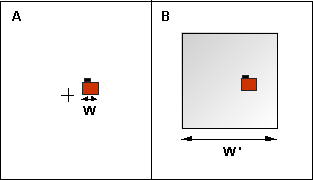
\includegraphics[width=\textwidth]{figures/ch2/princeSelection}
		\caption[\emph{Prince} dans un cas pratique]{Application de la technique \emph{Prince} à un cas de sélection pratique, avec pour cible une icône d'aire non nulle. Crédit : \cite{kabbash1995prince}.}
		\label{fig:princeSelection}
	\end{figure}
	
	La technique \emph{Prince} présente également l'avantage de permettre la sélection de plusieurs cibles d'un coup si elles sont incluses dans le curseur, mais cet avantage reflète une limitation de \emph{Prince}, car il peut dans ces cas-là y avoir ambiguïté si l'utilisateur ne souhaite sélectionner qu'une seule cible.
	
	\subsection{\emph{(Sticky) Area Cursor}, \emph{stickiness} et adaptativité}
		\subsubsection{Adaptativité}
	Une solution à ce problème d'ambiguïté est proposée par Worden \emph{et al.}~\cite{worden1997making} : lorsqu'un curseur zonal recouvre plusieurs cibles, le curseur devient en pratique un curseur ponctuel, et seul son centre est actif, comme l'illustre la figure~\ref{fig:areaCursor}.
	
	\begin{figure}[ht]
		\centering
		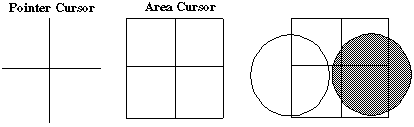
\includegraphics[width=\textwidth]{figures/ch2/areaCursor}
		\caption[\emph{Area Cursor} avec \emph{hot spot}]{Un curseur zonal dont seul le centre, marqué par l'intersection de deux segments, demeure actif lorsque le curseur chevauche plusieurs cibles. Crédit : \cite{worden1997making}.}
		\label{fig:areaCursor}
	\end{figure}
	
	Cette technique simple permet de tirer parti des avantages d'un curseur zonal quand la densité de cibles est suffisamment faibles, sans pour autant souffrir de ses inconvénients lorsqu'elle est élevée, puisque l'on revient alors à un simple curseur ponctuel.
	
		\subsubsection{\emph{Stickiness}}
	À cette solution, Worden \emph{et al.} ont ajouté l'usage de \emph{stickiness} adaptative pour les icônes. Un curseur est dit \emph{sticky} si, lorsqu'il s'approche d'une icône, celle-ci devient « collante ». En pratique, le ratio de sensibilité du curseur (la quantité du curseur par rapport à la quantité de mouvement du périphérique de saisie) diminue, ce qui permet d'une part de ralentir le curseur automatiquement, et d'autre part d'affiner les mouvements correctifs permettant la sélection d'une cible lors de son approche.
	
	Le problème des cibles collantes est que lorsque leur densité est élevée, donc en présence de nombreux distracteurs, la trajectoire du curseur se trouve fortement perturbée par ceux-ci, ce qui peut être contre-productif, ou du moins limiter les bénéfices de cette technique. La solution proposée par Worden \emph{et al.} est de ne rendre les cibles collantes que lorsque le curseur est à moins de 30~\%{} de la vitesse maximale qu'il a atteinte au cours de la tâche de sélection courante. L'hypothèse est qu'une sélection commence par une phase de mouvement très rapide et ample, suivie de petits mouvements correctifs plus lents, et que le curseur sera donc relativement lent près de la cible réellement visée par l'utilisateur.
	
	L'\emph{Area cursor}, en particulier complémenté par des cibles collantes et un gain adaptatif, permet un gain de performances important, en particulier avec des utilisateurs âgés, comme le détaille le tableau~\ref{tab:areaCursor}.
	
	\begin{table}
	\begin{tabular}{l c c c c}
										& \multicolumn{2}{c}{Jeunes}	&	\multicolumn{2}{c}{Âgés}			\\
										& Temps (ms)	& Taux de succès	& Temps (ms)	& Taux de succès	\\
		Pointeur seul					& 759			& 95,0				& 1893			& 95,0				\\
		Pointeur collant				& 712			& 97,4				& 1869			& 96,3				\\
		Pointeur adaptatif				& 743			& 97,7				& 1485			& 95,5				\\
		\emph{Area cursor} seul			& 639			& 96,9				& 1658			& 96,3				\\
		\emph{Area cursor} collant		& 596			& 97,9				& 1596			& 97,7				\\
		\emph{Area cursor} adaptatif	& 591			& 99,0				& 1203			& 97,9				\\
	\end{tabular}
	\caption{Performances mesurées pour un \emph{Area cursor} avec des cibles collantes, ainsi qu'avec des cibles collantes et un gain adaptatif en fonction de la vitesse du curseur. Les résultats sont comparés avec un curseur ponctuel dans les mêmes conditions, avec des sujets jeunes (23,4 ans en moyenne) et plus âgés (70,1 ans en moyenne). Les performances sont rapportées par le temps de sélection ainsi que le taux de succès (pourcentage de sélections réussies). Le curseur zonal avec cibles collantes et gain adaptatif permet les meilleures performances, tant avec des sujets jeunes que plus âgés, mais c'est au sein du second groupe que l'apport est le plus important. Données tirées de~\cite{worden1997making}.}
	\label{tab:areaCursor}
	\end{table}
	
	\subsection{Inconvénients}
	Le principal inconvénient d'un curseur zonal se présente lorsque la densité de cibles potentielles est élevée. Si deux cibles sont séparées d'une distance inférieure à la taille de la zone de sélection, il peut être difficile de choisir parmi les deux. Ce problème est illustré par la figure~\ref{fig:bubble}. Il est possible de partiellement pallier ce problème en utilisant une zone plus petite, mais en plus de réduire l'efficacité de la technique, ce n'est certain de fonctionner que si l'on connaît la distance minimale entre deux cibles \emph{a priori}. La figure~\ref{fig:areaCursor} présente une solution possible, qui consiste à n'utiliser que le centre du curseur, mais cela implique la perte de l'avantage fourni par un curseur zonal.

\section{\emph{Bubble Cursor}}
	\subsection{Principe et avantages}
	La technique \emph{Bubble Cursor} consiste à agrandir dynamiquement un curseur zonal (représenté par un disque) jusqu'à ce qu'il atteigne la cible la plus proche. Mathématiquement, cela revient à construire un diagramme de Voronoï des cibles et à s'appuyer dessus pour la sélection : le \emph{Bubble Cursor} est toujours dans une et une seule cellule du diagramme, et peut sélectionner la cible correspondante, comme l'illustrent les figures~\ref{fig:bubble} et~\ref{fig:voronoi}. De fait, dans sa version pure, il n'est capable de sélectionner que des cibles, pas l'espace entre celles-ci. Grossman et Balakrishnan ont montré que les performances de sélection avec le \emph{Bubble Cursor} suivent la loi de Fitts, à condition de remplacer la largeur de la cible par sa largeur effective, c'est-à-dire la largeur de sa cellule dans le diagramme de Voronoï~\cite{grossman2005bubble}, cf. la figure~\ref{fig:bubbleResults}. Le \emph{Bubble Cursor} peut être mis en œuvre en 2D aussi bien qu'en 3D~\cite{vanacken2007exploring}.	
		
	\begin{figure}[ht]
		\centering
		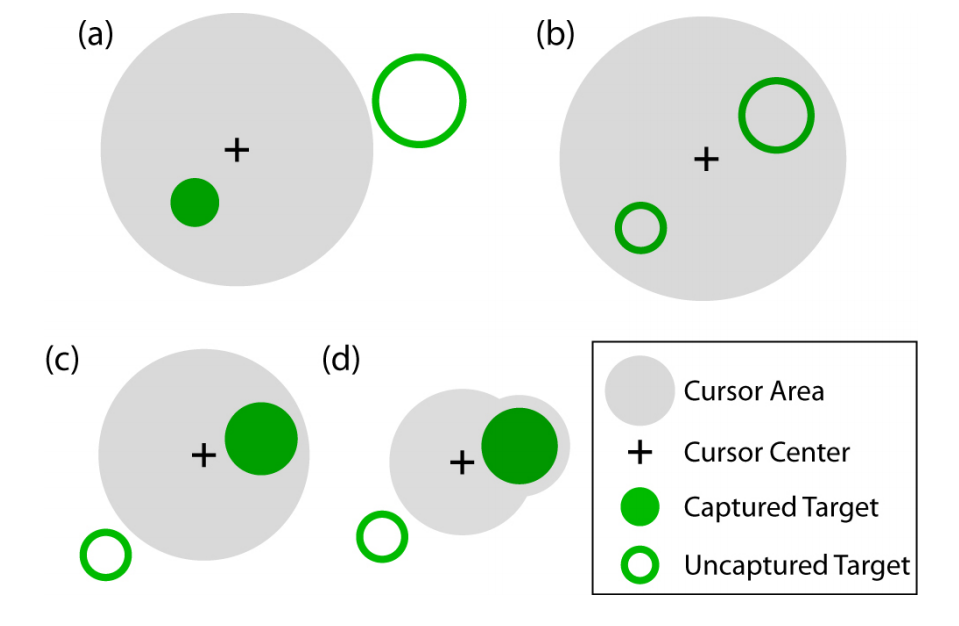
\includegraphics[width=\textwidth]{figures/ch2/bubble}
		\caption{Illustration du fonctionnement de la technique \emph{Bubble Cursor} (a, c, d) par opposition à un curseur zonal (b). Dans le cas b, le curseur zonal ne permet pas aisément de choisir entre les deux cibles qui se trouvent dans la zone de sélection. Mais le \emph{Bubble Cursor} s'adapte (c et d). Dans le cas (d), la cible n'est pas entièrement recouverte par le curseur, le disque du curseur, mais elle l'est partiellement, et pour représenter visuellement que c'est suffisant à sa sélection, le curseur est localement étendu pour l'englober. Crédit : \cite{grossman2005bubble}.}
		\label{fig:bubble}
	\end{figure}
	
	\begin{figure}[ht]
		\centering
		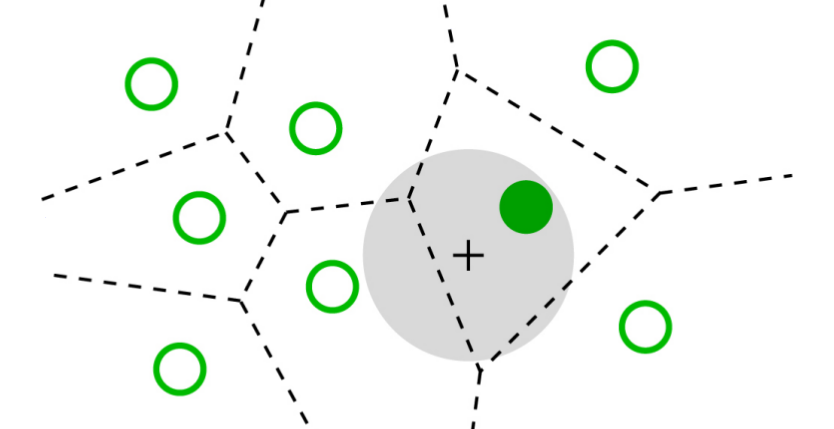
\includegraphics[width=\textwidth]{figures/ch2/voronoi}
		\caption{Diagramme de Voronoï définissant les cellules associées à chaque cible. Un diagramme de Voronoï est un découpage du plan (pavage) en cellules à partir d'un ensemble discret de points appelés « germes ». Chaque cellule enferme un seul germe, et forme l'ensemble des points du plan plus proches de ce germe que de tous les autres. La cellule représente en quelque sorte la « zone de proximité » du germe. Ici, les frontières d'activation de chaque cible, donc sa largeur effective, sont définies par sa cellule. Crédit : \cite{grossman2005bubble}.}
		\label{fig:voronoi}
	\end{figure}

	\begin{figure}[ht]
		\centering
		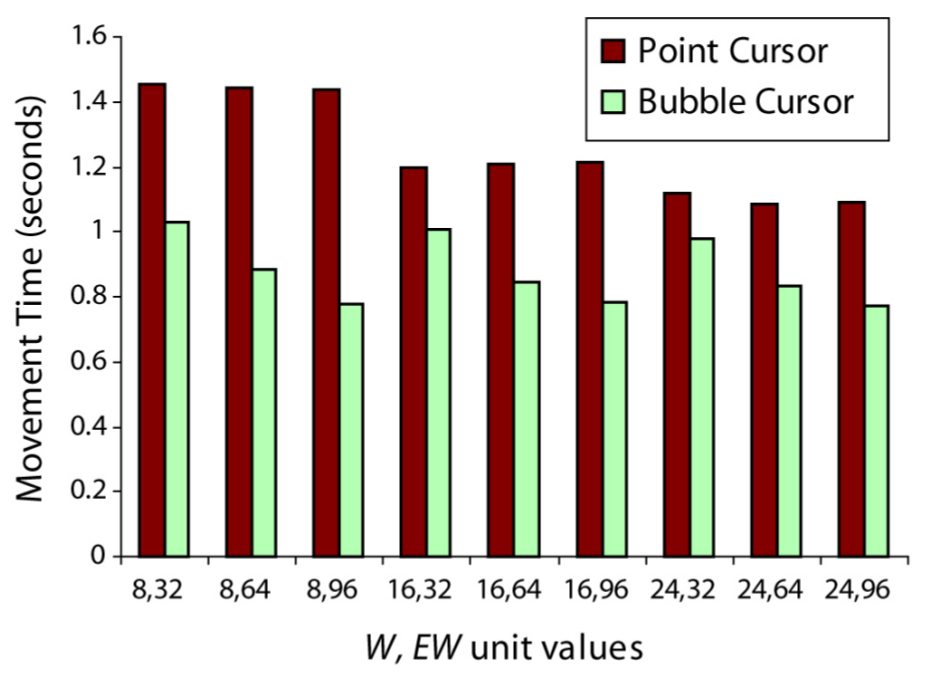
\includegraphics[width=\textwidth]{figures/ch2/bubbleResults}
		\caption{Temps mesuré pour atteindre la cible avec et sans le \emph{Bubble Cursor}, en fonction de $W$ et $EW$, où $W$ représente la largeur réelle de la cible, et $EW$ sa largeur effective, c'est-à-dire la taille de sa cellule de Voronoï. On constate que le \emph{Bubble Cursor} améliore les performances, et qu'il dépend de la largeur effective des cibles bien plus que de leur largeur réelle. Crédit : \cite{grossman2005bubble}.}
		\label{fig:bubbleResults}
	\end{figure}

	\subsection{Inconvénients}
	Un inconvénient de cette technique est le fait que le curseur peut rapidement croître et décroître à mesure qu'il s'approche et s'éloigne de plusieurs cibles successives. Cela peut représenter une source de distraction visuelle, en particulier quand les cibles elles-mêmes sont mobiles, \emph{a fortiori} si elles sont rapides. De plus, attendu que le \emph{Bubble Cursor} agrandit la largeur effective des cibles à la mesure de leur cellule de Voronoï, il est moins efficace en environnement dense, où les cellules de Voronoï sont plus petites. Le \emph{Bubble Cursor} montre donc ses limites face à des cibles potentielles nombreuses, mobiles et rapides.
	
	Un autre inconvénient (potentiellement majeur) du \emph{Bubble Cursor} est intrinsèquement lié à son mode de fonctionnement : il partage l'espace de sélection en un diagramme de Voronoï, où toute partie de l'espace fait partie de la zone de sélection d'une cible. Par conséquent, il n'existe plus d'espace « vide » dans lequel on pourrait utiliser le périphérique de saisie pour effectuer une opération indépendante des cibles, par exemple ouvrir un menu contextuel.

\section{\emph{DynaSpot}}
	\subsection{Principe}
	Cette dernière lacune du \emph{Bubble Cursor} est une des raisons d'être de \emph{DynaSpot}~\cite{chapuis2009dynaspot}. Celle-ci est une technique qui relie l'aire du curseur à sa vitesse. Le curseur conserve sa taille normale lorsqu'il est lent, mais croît et affecte une plus grande surface quand il se déplace plus vite. De fait il suffit de ralentir pour ramener le curseur à un comportement « normal » et pouvoir sélectionner de l'espace vide, par exemple pour ouvrir un menu contextuel, ou agir directement sur l'espace vide, comme l'illustre la figure~\ref{fig:dynaSpot}.
	
	\begin{figure}[H]
		\centering
		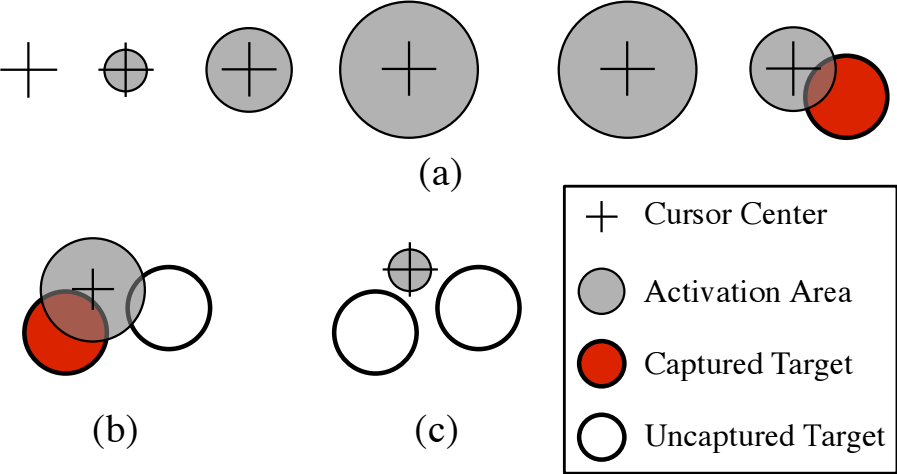
\includegraphics[width=\textwidth]{figures/ch2/dynaSpot}
		\caption{(a) La zone d'activation de \emph{DynaSpot} est couplée à la vitesse du curseur : plus celui-ci est rapide, plus celle-là est grande. (b) Plusieurs objets coupent la zone de sélection : la cible la plus proche du curseur est en surbrillance et sélectionnée. (c) Quand la zone de sélection ne touche aucun objet, il est possible de sélectionner l'espace vide, par exemple pour ouvrir un menu contextuel. Crédit : \cite{chapuis2009dynaspot}.}
		\label{fig:dynaSpot}
	\end{figure}
	
	Il n'est donc pas nécessaire de désactiver \emph{DynaSpot} ou de changer de mode explicitement. En ceci, \emph{DynaSpot} comble une des lacunes du \emph{Bubble Cursor}. Chapuis \emph{et al.}~\cite{chapuis2009dynaspot} ont montré que dans la plupart des cas, les performances de \emph{DynaSpot} sont similaires à celles du \emph{Bubble Cursor}. Ces résultats sont résumés dans la figure~\ref{fig:dynaResults}.
	 
	\begin{figure}[H]
		\centering
		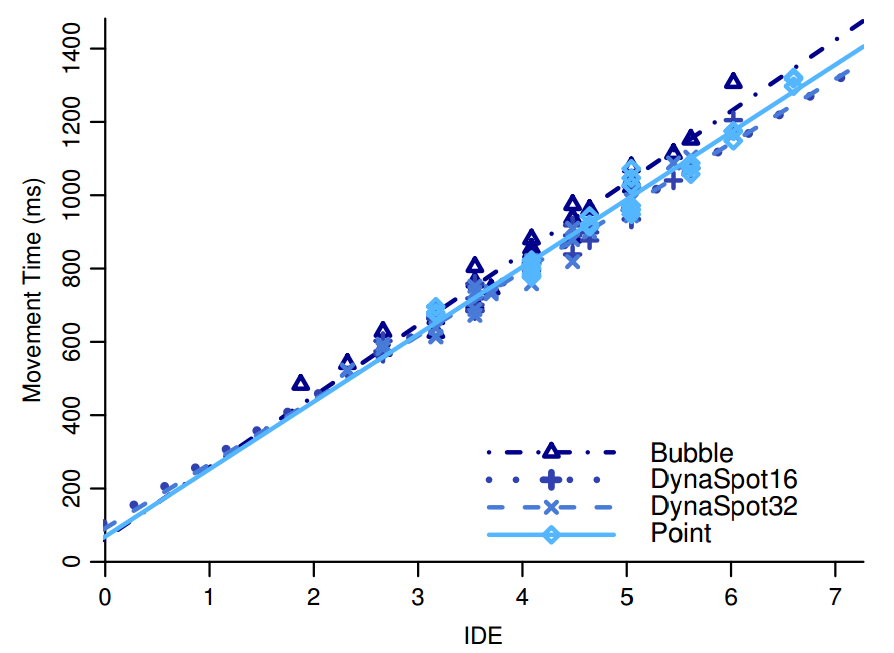
\includegraphics[width=\textwidth]{figures/ch2/dynaResults}
		\caption{Les performances (en temps de sélection) du \emph{BubbleCursor}, de \emph{DynaSpot} (dans deux versions paramétrées différemment) et d'un curseur ordinaire, en fonction de l'indice de difficulté. Celui-ci est calculé en fonction de la largeur de la cible pour le curseur ordinaire, mais en fonction de la largeur effective pour le \emph{Bubble Cursor} et \emph{DynaSpot}. Crédit : \cite{chapuis2009dynaspot}.}
		\label{fig:dynaResults}
	\end{figure}

	Attendu que la croissance et la décroissance du curseur sont à la fois lentes et prévisibles avec cette technique, le niveau de distraction visuelle est faible. Par ailleurs, il n'est pas nécessaire de connaître la position des cibles potentielles pour appliquer \emph{DynaSpot}, qui ne dépend que de la vitesse du curseur. En cela, cette technique permet de pallier deux autres inconvénients du \emph{Bubble Cursor}.

	\subsection{Inconvénients}
	Le principal inconvénient de cette technique est précisément le fait que le curseur ne tient pas compte des cibles. Par conséquent, à vitesse élevée, sa surface peut en recouvrir plusieurs, et il ne peut déterminer laquelle est la bonne. Il est donc nécessaire de ralentir et d'attendre que le curseur rapetisse suffisamment pour ne toucher qu'une cible. En pratique, cela se produit assez rapidement, et pour les cibles statiques ce n'est pas vraiment gênant. Mais si les cibles sont mobiles, et \emph{a fortiori} rapides, le curseur ne peut s'arrêter, et il peut même être impossible à l'utilisateur de ralentir suffisamment pour que le curseur retrouve une taille permettant la sélection. Ainsi, de même que pour le \emph{Bubble Cursor}, la densité et la vitesse des cibles posent de sérieux problèmes.

	On pourrait toutefois envisager une sélection en deux temps (en cascade) : l'utilisateur pré-sélectionnerait plusieurs cibles lorsque le curseur est gros et rapide, puis devrait choisir parmi les cibles touchées laquelle il veut. Naturellement, le processus de sélection en deviendrait plus lourd et plus long, et pourrait nécessiter de stopper (ou ralentir) les cibles après l'étape de pré-sélection pour que la sélection finale soit réalisable, ou bien encore de zoomer fortement sur l'espace pré-sélectionné. Cette dernière solution est intéressante sur le papier mais pourrait s'avérer peu pratique si les cibles de l'espace pré-sélectionné ont des directions opposées et sont suffisamment rapides pour forcer un « dézoom » avant que la sélection finale ne puisse avoir lieu.
	
\section{\emph{Silk Cursor}}
	\subsection{Principe et avantages}
	~\cite{zhai1994silk}
	
	\subsection{Inconvénients}
	
\section{\emph{Target/Bubble Ghost}}
	\subsection{Principe et avantages}
	\emph{Target Ghost}~\cite{hasan2011comet} est une technique qui repose sur un déclenchement délibéré. Quand elle est déclenchée par l'utilisateur, \emph{Target Ghost} duplique toutes les cibles potentielles. Une des copies devient statique et reste opaque, tandis que l'autre demeure mobile mais est rendue semi-transparente, comme l'illustre la figure~\ref{fig:targetGhost}.
	
	\begin{figure}[H]
		\centering
		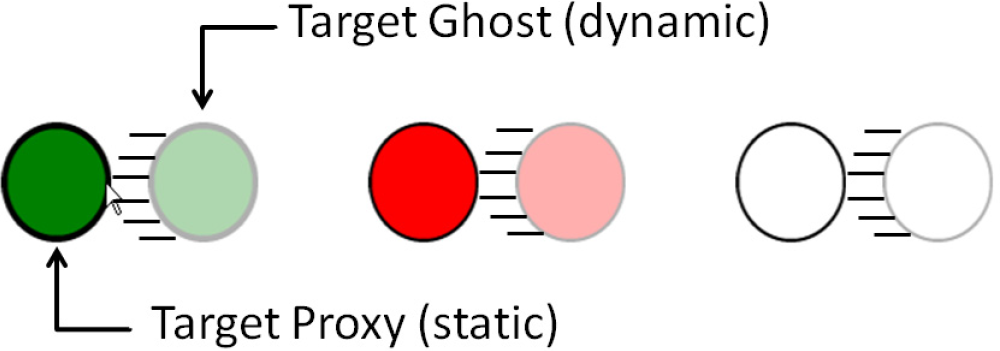
\includegraphics[width=\textwidth]{figures/ch2/targetGhost}
		\caption[La technique \emph{Target Ghost}]{(Les flèches et annotations ont été ajoutées à l'image pour l'illustrer). La technique \emph{Target Ghost} avec un curseur basique. Quand elle est « \emph{ghostée} » la cible originale voit la saturation de sa couleur baisser (en tant que fantôme) mais elle poursuit sa trajectoire. Un proxy beaucoup plus net de l'objet demeure figé à la position qu'il occupait lorsque la touche \emph{Maj} a été pressée, et il peut être sélectionné relativement aisément. D'ailleurs, seul le proxy peut être sélectionné, au contraire du fantôme de la cible. Crédit : \cite{hasan2011comet}.}
		\label{fig:targetGhost}
	\end{figure}
	
	L'utilisateur peut ensuite sélectionner la version statique et opaque de la cible, qui sert de proxy pour sa jumelle mobile. Cela permet de ramener une tâche de sélection de cible mobile à une simple sélection de cible statique. Naturellement, cela facilite considérablement les choses, ce qui permet d'améliorer significativement les temps de sélection et, dans une plus grande mesure encore, les taux d'erreur, comme le montrent les graphiques des figures~\ref{fig:cometGhostTimes}, \ref{fig:cometGhostErrors} et~\ref{fig:cometGhostPredictability}.

	\begin{figure}[H]
		\centering
		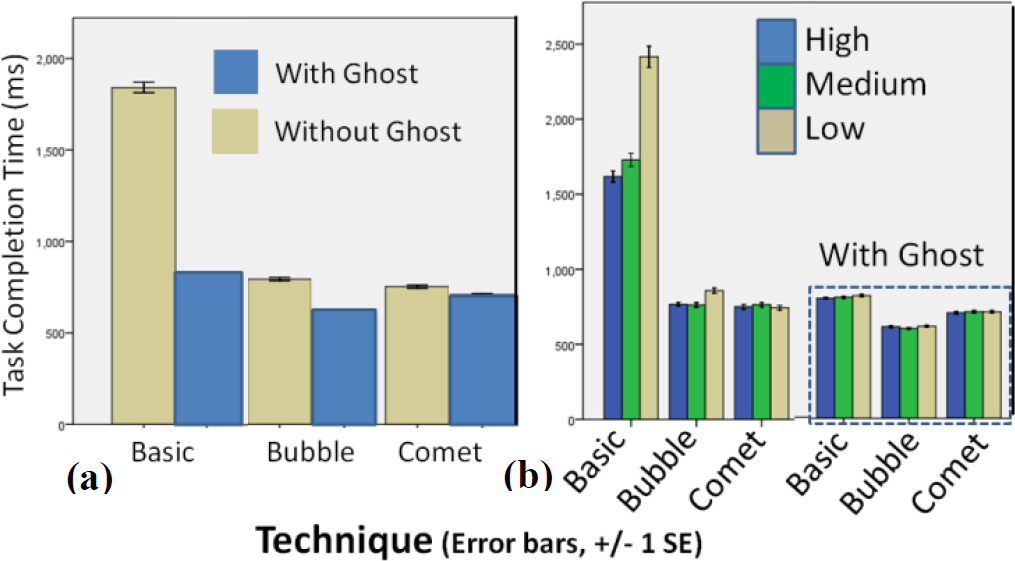
\includegraphics[width=\textwidth]{figures/ch2/cometGhostPredictability}
		\caption[\emph{Comet/Ghost}, prévisibilité et résultats]{Temps de complétion de la tâche, (a) : en fonction des types de curseur, avec ou sans \emph{Ghost}, (b) : en fonction de la prévisibilité du chemin pris par la cible. La technique \emph{Comet} est décrite dans la section suivante. Crédit : \cite{hasan2011comet}.}
		\label{fig:cometGhostPredictability}
	\end{figure}
	
		\begin{figure}[H]
		\centering
		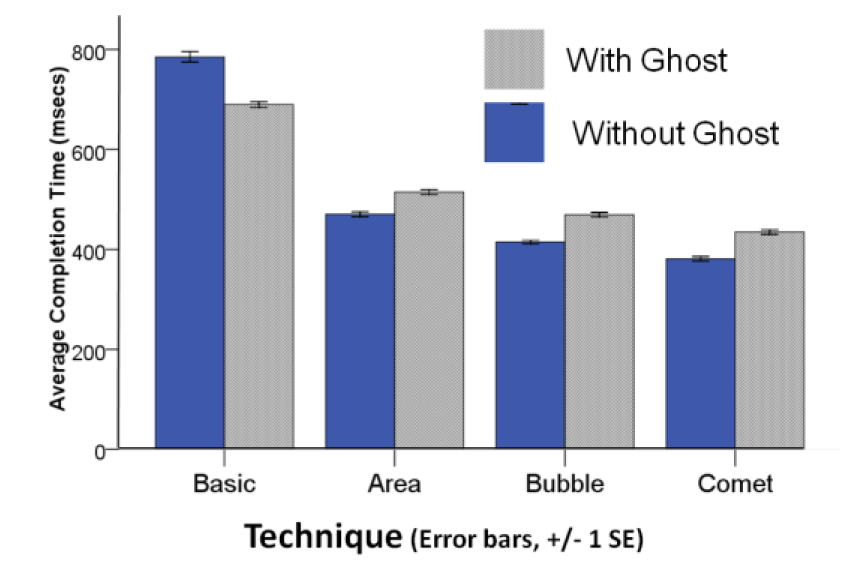
\includegraphics[width=\textwidth]{figures/ch2/cometGhostTimes}
		\caption[\emph{Comet/Ghost}, temps de sélection]{Temps de complétion de la tâche de sélection, avec plusieurs techniques (curseur basique, curseur zonal, \emph{Bubble Cursor} et \emph{Comet}), avec et sans \emph{Ghost}. On constate que l'usage d'un fantôme est bénéfique sur un curseur basique, mais néfaste dans tous les autres cas. Par ailleurs, \emph{Comet} offre les meilleures performances. Il ne s'agit cependant ici que du temps de sélection. La technique \emph{Comet} est décrite dans la section suivante. Crédit : \cite{hasan2011comet}.}
		\label{fig:cometGhostTimes}
	\end{figure}
	
	\begin{figure}[H]
		\centering
		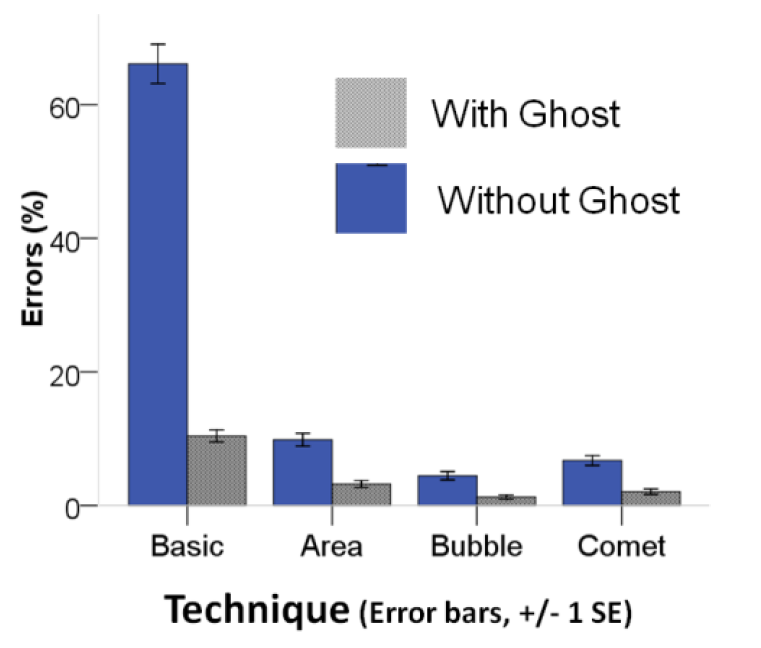
\includegraphics[width=\textwidth]{figures/ch2/cometGhostErrors}
		\caption[\emph{Comet/Ghost}, taux d'erreur]{Taux d'erreur pour la tâche de sélection, avec plusieurs techniques (curseur basique, curseur zonal, \emph{Bubble Cursor} et \emph{Comet}), avec et sans \emph{Ghost}. On constate que l'usage d'un fantôme est très bénéfique dans tous les cas, même s'il augmente le temps de sélection lorsqu'une meilleure technique que le curseur basique est utilisée. La technique \emph{Comet} est décrite dans la section suivante. Crédit : \cite{hasan2011comet}.}
		\label{fig:cometGhostErrors}
	\end{figure}
		
	De plus, cette technique n'affectant que les cibles, elle peut être combinée à une technique de curseur, ce qui fut d'ailleurs fait avec le \emph{Bubble Cursor}, pour une combinaison baptisée \emph{Bubble Ghost}~\cite{hasan2011comet}.
		
	\subsection{Inconvénients}
	Là encore, l'inconvénient principal de cette technique est l'augmentation de l'encombrement visuel, puisque le nombre de cibles affichées double, même si la moitié d'entre elles sont semi-transparentes. Le \emph{ghosting} peut par ailleurs aggraver le problème d'occultation : en effet, si une cible mobile passe derrière un objet statique ou une autre cible potentielle, déclencher \emph{Target/Bubble Ghost} à cet instant aurait pour effet de prolonger indéfiniment l'occultation de cette cible. Ce problème est d'autant plus gênant que la densité de cibles potentielles est élevée.
		
	L'utilisation d'un proxy peut aussi être gênante dans un contexte immersif avec un périphérique de saisie permettant une correspondance à l'échelle 1 entre l'espace moteur et l'espace virtuel, en particulier si la sélection a pour but de permettre une manipulation de l'objet saisi. C'est notamment le cas pour les simulations de dynamique moléculaire, qui impliquent d'envoyer des forces au système simulé, avec un retour (pseudo-)haptique pour l'utilisateur.

\section{\emph{(Bubble) Comet}}
	\subsection{Principe et avantages}
	Avec \emph{Comet}~\cite{hasan2011comet}, chaque cible potentielle laisse derrière elle une traînée (ou queue) qui peut être sélectionnée à la place de la cible elle-même, comme le montre la figure~\ref{fig:comet}.
	
	\begin{figure}[H]
		\centering
		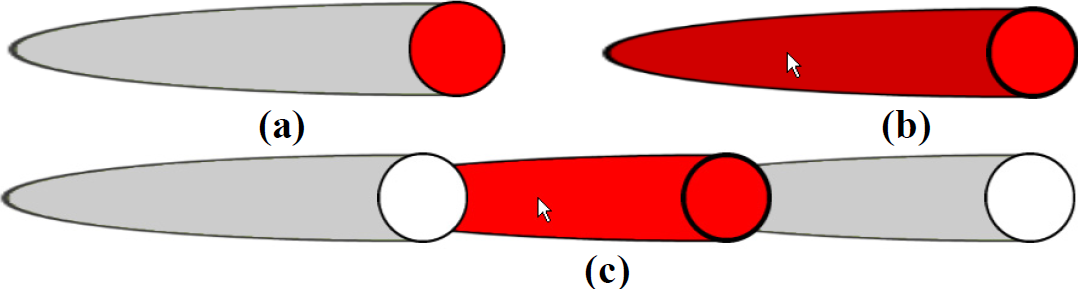
\includegraphics[width=\textwidth]{figures/ch2/comet}
		\caption[La technique \emph{Comet}]{(a) La cible et sa queue de comète. (b) La queue est mise en surbrillance lorsque le curseur passe dessus. (c) Les queues peuvent être recouvertes par les cibles ajdacentes. Crédit : \cite{hasan2011comet}.}
		\label{fig:comet}
	\end{figure}	
	
	Cela revient à augmenter la taille effective des cibles. Attendu que cela s'applique aux cibles et pas aux curseurs, \emph{Comet} peut être combinée à une technique de curseur, par exemple le \emph{Bubble Cursor} ou \emph{DynaSpot}. Hasan \emph{et al.} ont montré que cette technique permet de significativement améliorer les temps de sélection et les taux d'erreur pour les cibles mobiles en 2D~\cite{hasan2011comet}, comme le montrent les résultats compilés sur les figures~\ref{fig:cometGhostTimes}, \ref{fig:cometGhostErrors} et~\ref{fig:cometGhostPredictability}.

	\subsection{Inconvénients}
	Cependant, \emph{Comet} ajoute un « encombrement » visuel important. En effet, à chaque cible vient s'ajouter une queue qui fait plusieurs fois sa taille. Étendue à la 3D, cette technique ferait logiquement usage de rendu volumique semi-transparent pour les queues de comètes, ce qui aurait probablement pour effet de porter l'encombrement visuel et donc l'occultation à des niveaux inacceptables, surtout dans des environnements denses. Un autre inconvénient de cette technique est qu'elle modifie la représentation visuelle des cibles, et en particulier de leur forme. Pour certaines applications, par exemple les simulations moléculaires (dans lequelles la perception des formes des molécules est absolument critique) ce point est particulièrement gênant. Par conséquent, la technique \emph{Comet} ne peut être retenue pour les environnements tridimensionnels denses.

	De surcroît, si son couplage à du \emph{ghosting} est parfois avantageux, comme nous l'avons vu plus haut, c'est au prix d'un encombrement visuel qui s'en trouve encore accru, à un point hélas inacceptable pour de nombreuses applications nécessitant la sélection de cibles mobiles en environnements particulièrement denses.

\section{\emph{AttachedShock}}
	\subsection{Principe et avantages}
	\emph{AttachedShock}~\cite{you2012attachedshock, you2014attachedshock}. est une technique développée pour répondre à un besoin plutôt spécifique à la réalité augmentée : la sélection d'objets « fuyants » : lorsqu'un utilisateur se déplace dans une direction (à pied ou dans un véhicule) les objets à côté desquels il passent quittent son champ de vision rapidement, et de plus en plus vite à mesure que qu'ils s'approchent des bords du champ de vision, comme l'illustre la figure~\ref{fig:as2dspeed}.
	
	\begin{figure}[H]
		\centering
		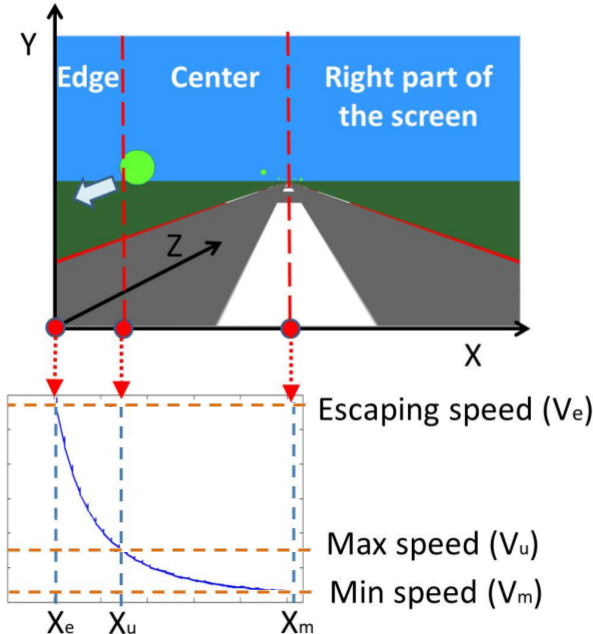
\includegraphics[width=\textwidth]{figures/ch2/as2dspeed}
		\caption[\emph{AttachedShock}, profil de vitesse]{Représentation de la vue d'un utilisateur utilisant un système de réalité augmentée dans une voiture, et fixant la route en face de lui. Des objets, ici représentés par des sphères vertes, attirent son attention. Ils sont fixés au sol, mais leur vitesse relative déterminée par rapport au référentiel de la voiture correspond à la vitesse de la voiture dans le référentiel terrestre. Si celle-ci est constante, alors la vitesse relative des objets l'est aussi ; pourtant, une fois projetée sur un écran 2D, elle varie considérablement en fonction de la distance de l'objet au centre de l'écran, comme l'illustre la courbe sous l'image. On peut parler de \emph{vitesse apparente}. Crédit : \cite{you2012attachedshock}.}
		\label{fig:as2dspeed}
	\end{figure}
	
	Pour faciliter la sélection de telles cibles sans trop augmenter l'encombrement visuel (\emph{clutter}) de la scène, les auteurs d'\emph{AttachedShock} ont choisi d'ajouter aux objets apparemment en mouvement une onde de choc, comme sur la figure~\ref{fig:asas}. Cette onde est augmente l'objet en facilite la sélection. \emph{AttachedShock} fait donc partie de la famille des techniques de sélection qui cherchent à faciliter la sélection en augmentant la taille effective des cibles. La sélection se fait en effet en « traversant » l'onde de choc d'un objet, ce qui permet aux utilisateurs d'effectuer un mouvement balistique sans avoir à ralentir comme ils le devraient avec une cible non augmentée.

	\begin{figure}[H]
		\centering
		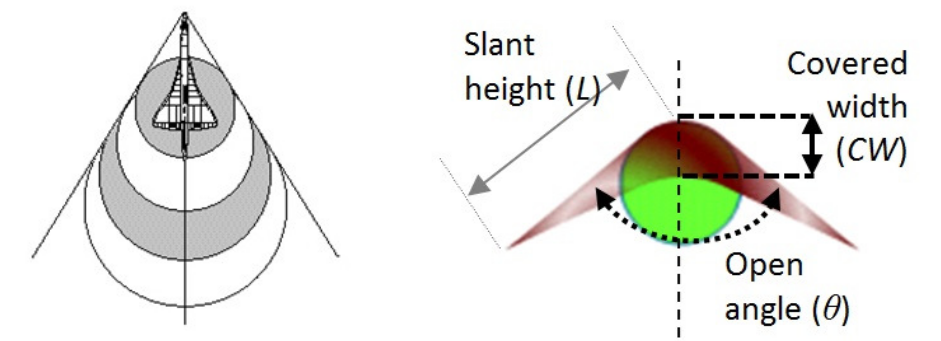
\includegraphics[width=\textwidth]{figures/ch2/asas}
		\caption[\emph{AttachedShock}, onde de choc]{À gauche, une représentation schématique de la réelle onde de choc d'un avion supersonique (un \emph{Concorde}). À droite, une cible mobile (la sphère verte) accompagnée de son onde de choc telle qu'elle est représentée par \emph{AttachedShock}. Cette onde vient augmenter la représentation visuelle de la cible afin d'en faciliter la sélection. Crédit : ~\cite{you2012attachedshock}.}
		\label{fig:asas}
	\end{figure}
	
Cette technique a pour particularité de le faire en limitant l'encombrement visuel et en optant pour une augmentation visuelle pouvant être perçue comme « naturelle » --- plus par habitude des ondes de choc qui se propagent dans l'eau que de celles générées par les avions supersoniques, sans doute. Les auteurs ont comparé \emph{AttachedShock} à d'autres techniques de référence, dont bien sûr un simple curseur de type « point » mais aussi un curseur zonal, ainsi que la technique \emph{Comet}, présentée plus haut.

La technique \emph{AttachedShock} s'est montrée meilleure que toutes les autres dans cette évaluation, quoique de peu pour le temps de sélection. Les résultats détaillés sont illustrés par la figure~\ref{fig:asRes}. Dans les conditions du protocole de test mis en place par les auteurs, \emph{AttachedShock} permet une sélection rapide et fiable par rapport aux techniques existantes, avec un encombrement visuel très contenu.
	
	\begin{figure}[H]
		\centering
		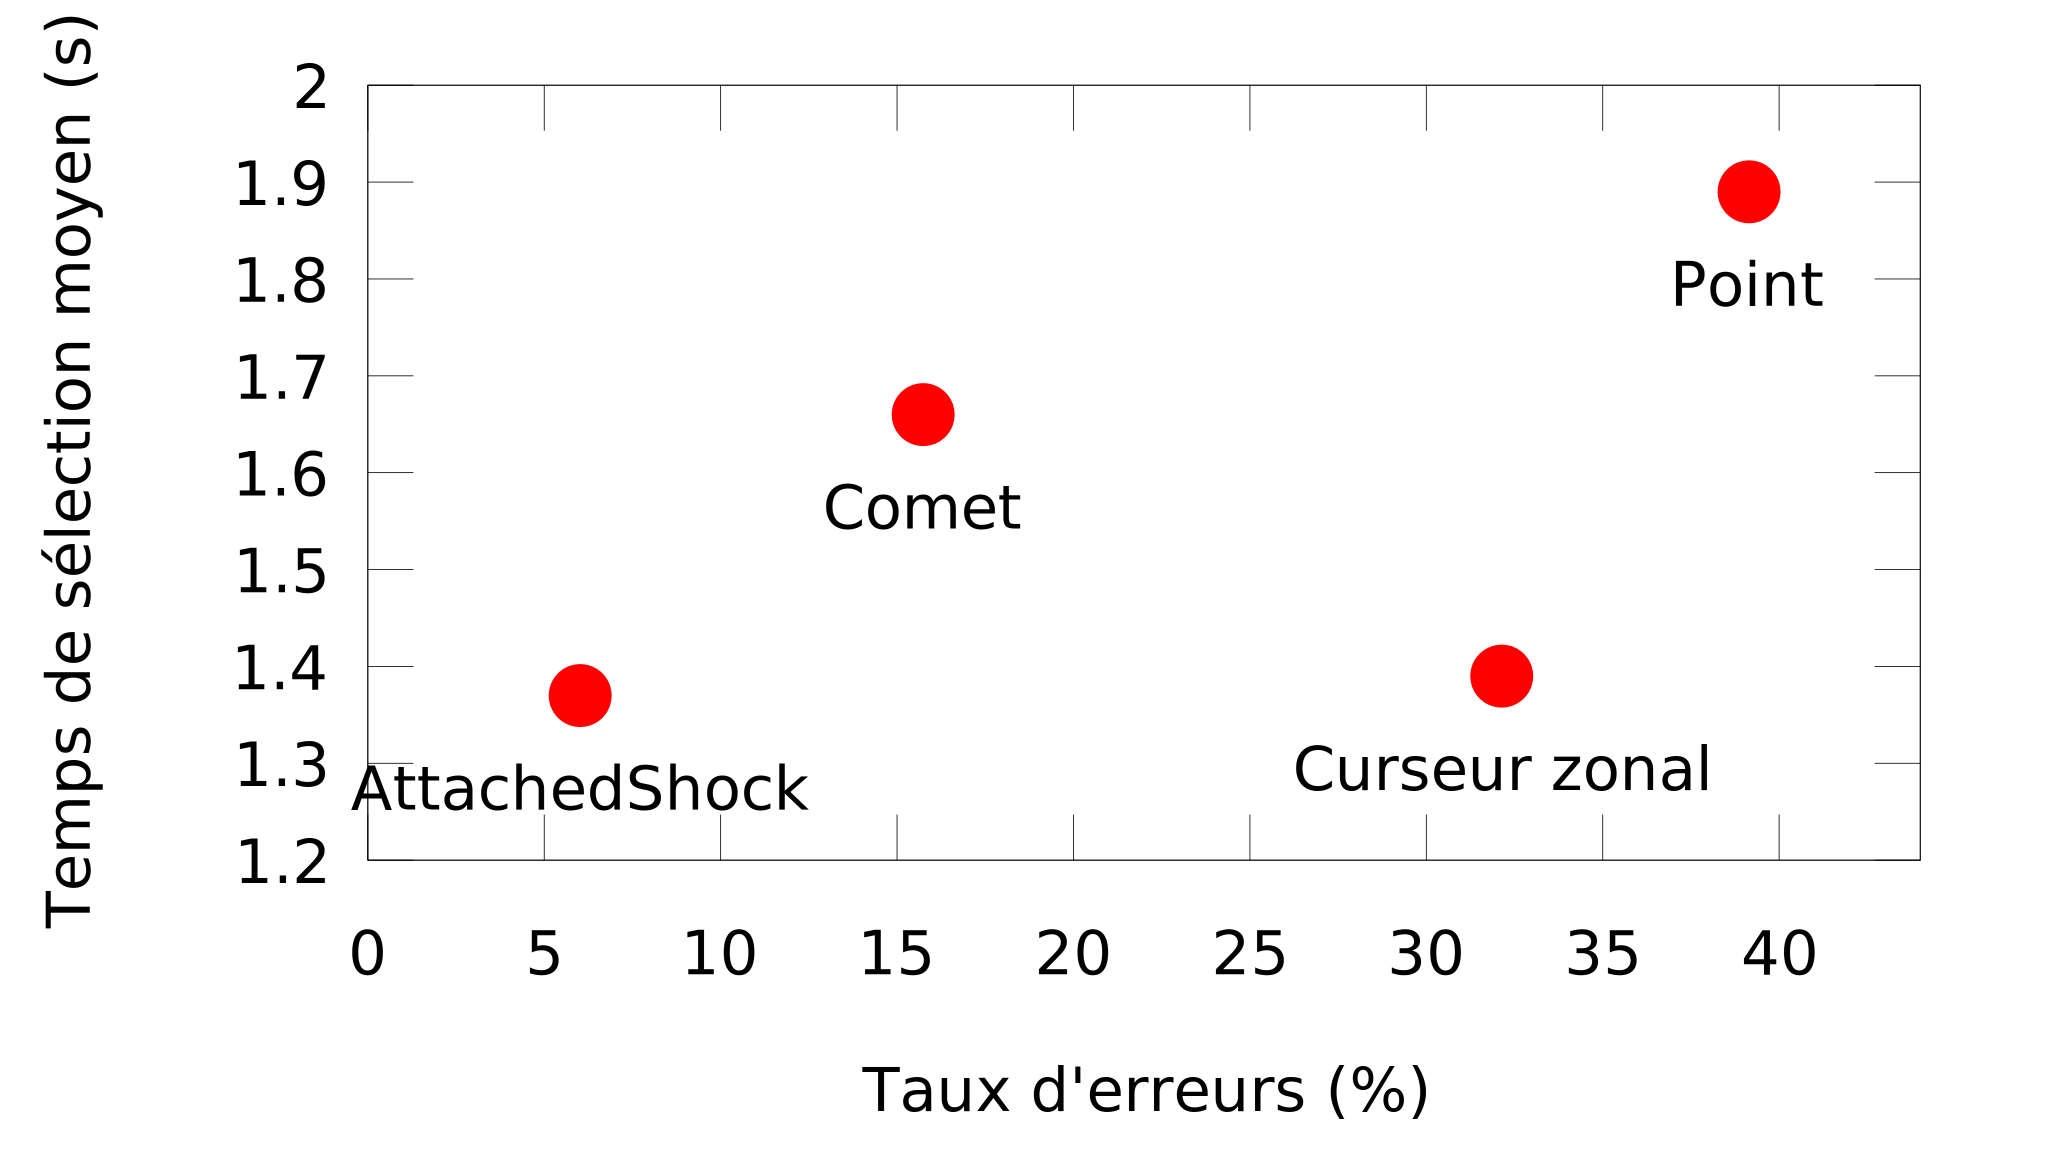
\includegraphics[width=\textwidth]{figures/ch2/asRes}
		\caption[\emph{AttachedShock}, performance]{Présentation des résultats obtenus par les auteurs d'\emph{AttachedShock} au cours de leur évaluation de cette technique. Le taux d'erreurs est en abscisse, et le temps de sélection en ordonnée. Une technique idéale serait donc à l'origine. \emph{AttachedShock} ne fait pas beaucoup mieux qu'un curseur zonal (\emph{Area}) en temps de sélection, mais s'illustre pas un taux d'erreur très bas, et par un temps de sélection moyen qui demeure le meilleur, même s'il est très proche de celui du curseur zonal. Résultats bruts tirés de~\cite{you2012attachedshock}.}
		\label{fig:asRes}
	\end{figure}

	\subsection{Inconvénients}
	\emph{AttachedShock} n'est toutefois pas sans limite. En effet, la densité de cibles testée par les auteurs est très faible, comme le montre la figure~\ref{fig:asDensity}. La technique n'ayant pas été évaluée avec une grande densité de cibles, il est impossible d'affirmer qu'elle fonctionnerait bien dans de telles conditions, mais l'on peut en douter compte tenu du fait qu'elle repose sur la possibilité qu'a l'utilisateur de se « contenter » de mouvements balistiques sans mouvements correctifs, ce qui serait bien difficile avec les nombreux obstacles que de nombreux distracteurs constitueraient.
	
	\begin{figure}[ht]
		\centering
		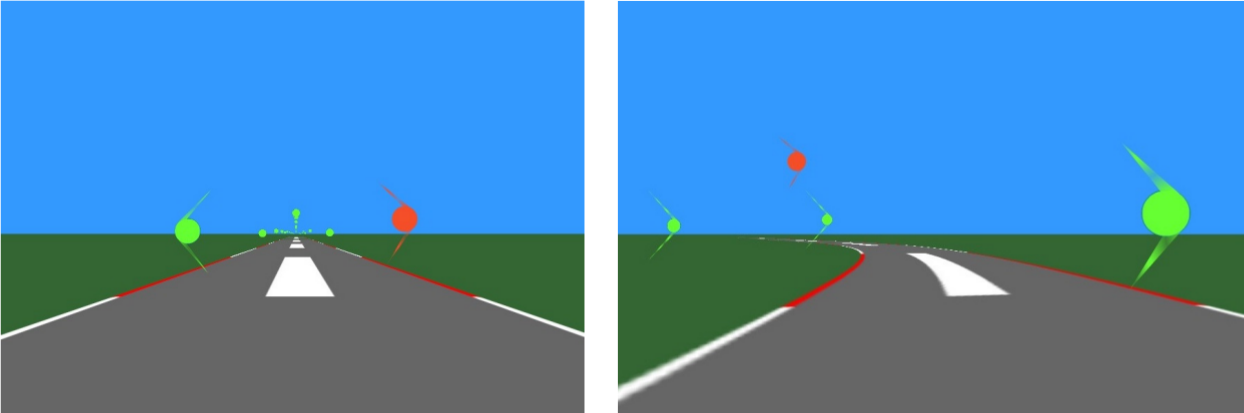
\includegraphics[width=\textwidth]{figures/ch2/asDensity}
		\caption[\emph{AttachedShock}, densité de cibles]{Captures d'écran du dispositif d'évaluation d'\emph{AttachedShock}. À gauche, l'expérience est menée sur un segment de route rectiligne ; à droite, sur un segment courbe. La sphère rouge est la cible à sélectionner, tandis que les vertes sont des distracteurs. On constate que les distracteurs sont peu nombreux et qu'il est relativement peu probable de « traverser » leur onde de choc en essayant d'atteindre cette de la cible. Crédit: \cite{you2012attachedshock}.}
		\label{fig:asDensity}
	\end{figure}
	
	En outre, dans cette évaluation les cibles sont fixées au sol, et donc ne se déplacent à l'écran qu'à l'horizontale. De fait, leurs ondes de choc se présentent toujours dans la même orientation. Or, dans bien des cas, les cibles peuvent changer de direction en cours de route, ce qui soumettrait logiquement ces ondes de choc à de fréquentes rotations. Dans ces condtions, déclencher un mouvement balistique pour traverser l'onde de choc sans mouvements correctifs serait sans doute beaucoup plus difficile.
	
	Ainsi, si \emph{AttachedShock} présente un intérêt certain pour la sélection de cibles mobiles peu nombreuses (avec peu de distracteurs) se déplaçant à l'horizontale, son efficacité en environnement dense et/ou avec des cibles changeant souvent de direction, \emph{a fortiori} de manière imprévisible, demeure à démontrer. Et compte tenu du fonctionnement de la technique, on peut même s'attendre à une chute significative de son efficacité relative dans ces conditions.

\section{\emph{Hold}}
	\subsection{Principe et avantages}
	Le principe de \emph{Hold}~\cite{hajri2011moving} est très simple : sur déclenchement explicite de la part de l'utilisateur, les cibles deviennent statiques, ce qui facilite considérablement leur sélection puisque cela revient à une simple sélection statique, modélisée par la loi de Fitts. Une particularité de cette technique est que les cibles peuvent être stoppées à tout moment par la pression d'un boutons, et « réactivées » en relâchant le bouton, à volonté. Ce fonctionnement est illustré par la figure~\ref{fig:hold}.
	
	\begin{figure}[ht]
		\centering
		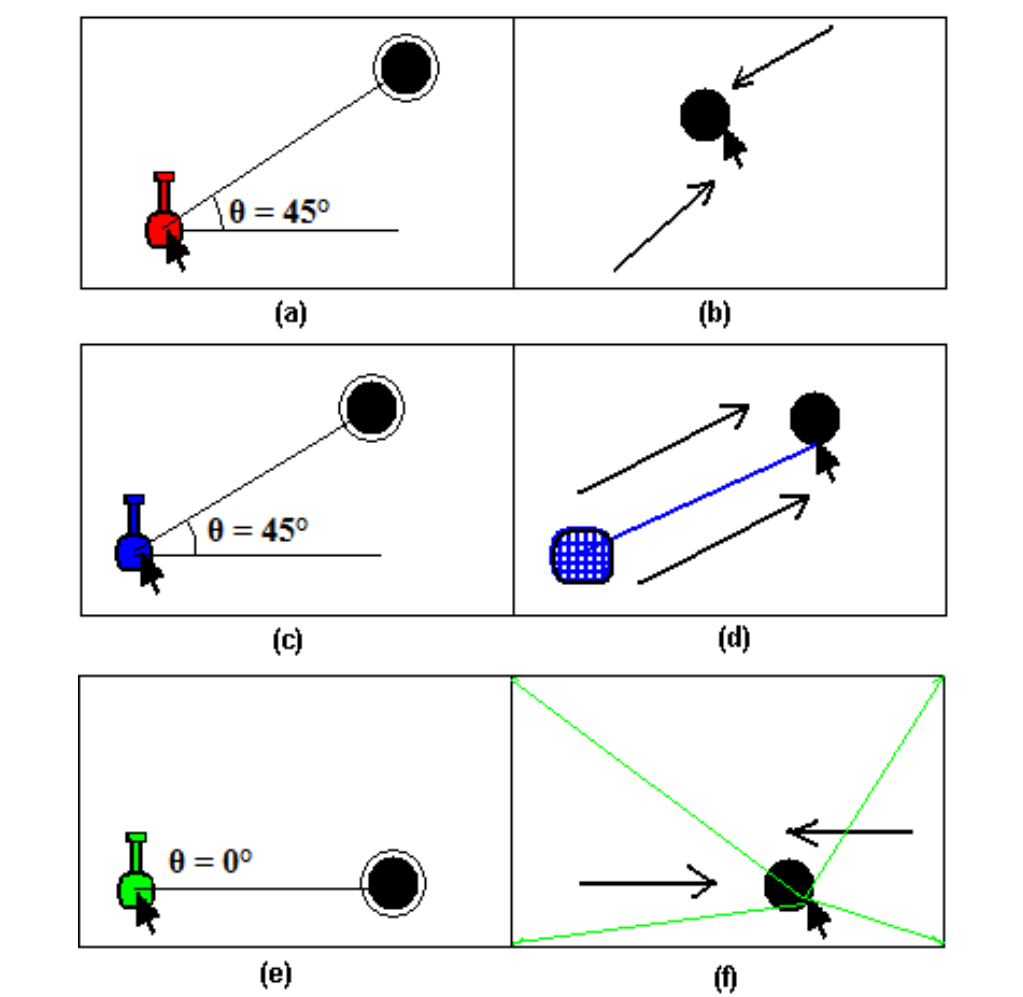
\includegraphics[width=\textwidth]{figures/ch2/hold}
		\caption[La technique \emph{Hold}]{Mode de fonctionnement de la technique \emph{Hold} telle qu'elle fut évaluée dans~\cite{hajri2011moving}. En haut (a,b) le système classique (baptisé \emph{Chase} par Al Hajri \emph{et al.}) : l'utilisateur positionne sa souris sur le flacon rouge pour déclencher la sélection, et doit ensuite cliquer sur le disque noir. Au milieu (c,d) la technique \emph{Hold} ; l'utilisateur doit cliquer sur le flacon bleu pour arrêter la cible, maintenir le bouton pressé, et ne le relâcher que sur le disque noir. En bas (e,f), l'utilisateur doit d'abord positionner sa souris sur le flacon vert, puis peut cliquer librement sur le disque, comme dans le premier cas, ou cliquer sur le flacon pour stopper la cible et relâcher le bouton dessus, comme dans le deuxième cas. Cette technique est appelée \emph{Hybrid} par les auteurs, et a l'avantage d'être plus flexible. En effet, elle permet à un utilisateur de laisser une cible se déplacer avant de la sélectionner, ce qui peut être avantageux si elle se dirige vers le curseur. Crédit : \cite{hajri2011moving}.}
		\label{fig:hold}
	\end{figure}
	
	Cela peut pallier le problème d'occultation inhérent à ce type de technique, qui survient si l'on stoppe le mouvement des objets lorsque la cible visée est occultée par un autre objet --- tout particulièrement dans un contexte 3D. On ajoutera que comme la plupart des techniques portant sur les cibles, \emph{Hold} peut être couplée à une technique de curseur, comme le \emph{Bubble Cursor} ou \emph{DynaSpot}, par exemple.
	
	En pratique, l'évaluation de la technique \emph{Hold} menée par Al Hajri \emph{et al.} montre qu'elle \emph{augmente} le temps de sélection, mais réduit le taux d'erreurs. Les sujets de l'évaluation ont expliqué aux auteurs qu'une fois la cible stoppée, ils ressentaient moins le besoin de se presser pour la sélectionner, vu que la tâche était devenue plus facile. De plus, \emph{Hold} nécessite de cliquer une première fois pour stopper la cible, puis de maintenir le bouton de la souris pressé jusqu'à le relâcher sur la cible, ce qui implique un effort supplémentaire et peut partiellemet expliquer ces résultats. Enfin, le nombre de clics montre que les sujets privilégient la rapidité sans \emph{Hold}, et la précision avec.
	
	On peut néanmoins se demander s'ils auraient été identiques si les utilisateurs avaient été plus encouragés à se dépêcher, par exemple en affichant un chronomètre, ou avec un système de points. Les temps de sélection mesurés en fonction des différents paramètres régissant le mouvement de la cible à sélectionner sont détaillés sur la figure~\ref{fig:holdRes}.
	
	\begin{figure}[H]
		\centering
		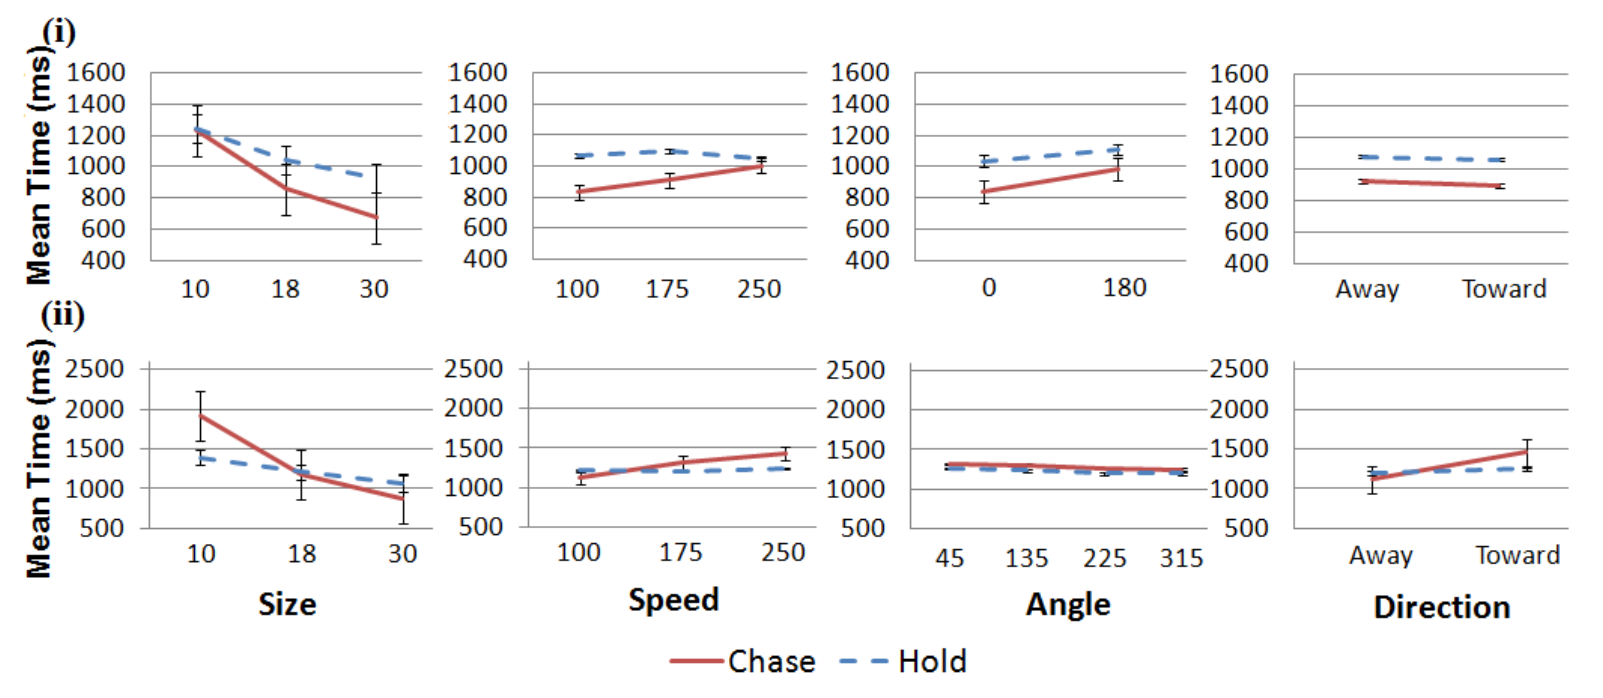
\includegraphics[width=\textwidth]{figures/ch2/holdRes}
		\caption[\emph{Hold} --- évaluation]{Résultats de l'évaluation de la technique \emph{Hold}. En haut, les résultats en 1D ; en bas, en 2D. Comme le prédit la loi de Fitts, la difficulté de sélection décroît avec la taille des cibles, et comme d'autres études l'ont montré, elle croît naturellement avec leur vitesse.  Crédit : \cite{hajri2011moving}.}
		\label{fig:holdRes}
	\end{figure}
	
	Toutefois, cette tendance générale s'inverse si l'on s'intéresse aux cibles les plus difficiles à sélectionner, c'est-à-dire celles qui sont rapides, petites, ou \emph{a fortiori} les deux à la fois, comme les résultats présentés sur la figure~\ref{fig:holdSFast} le montrent. C'est assez logique puisque la vitesse en particulier n'a que très peu d'incidence sur la difficulté de sélection avec \emph{Hold}, puisqu'elle s'annule dès que l'utilisateur délenche l'arrêt de la cible. La taille conserve son influence décrite par la loi de Fitts, mais son interaction avec la vitesse disparaît presque totalement.
	
	\begin{figure}[H]
		\centering
		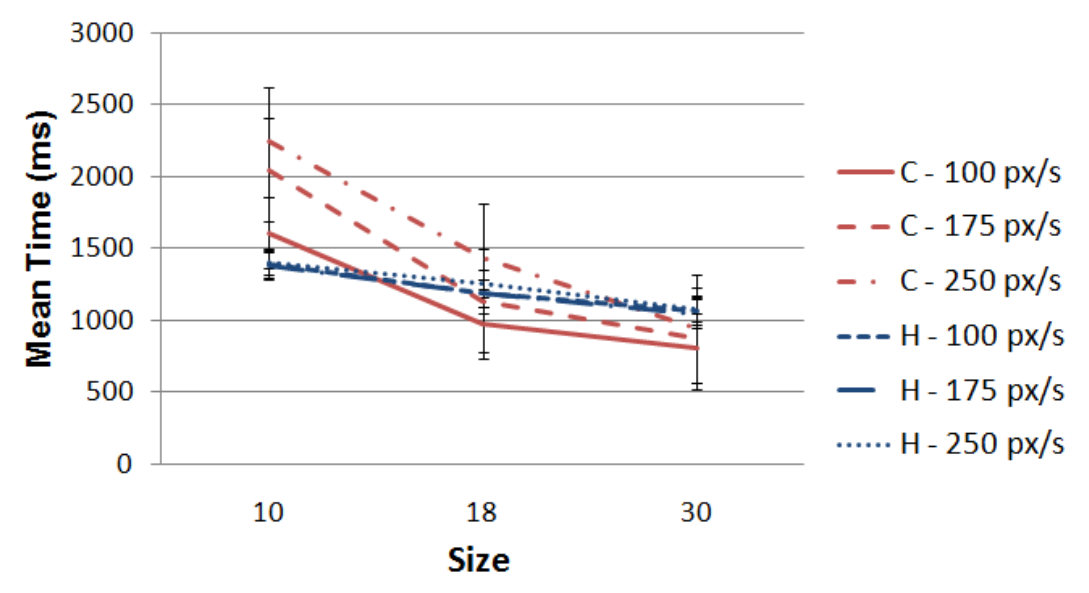
\includegraphics[width=\textwidth]{figures/ch2/holdSFast}
		\caption[\emph{Hold} --- petites cibles rapides]{Résultats de l'évaluation de la technique \emph{Hold} en fonction de la taille et de la vitesse de la cible. En rouge (légende \emph{C}) sont notés les temps de sélection de la technique \emph{Chase}, c'est-à-dire la sélection classique ; en bleu (légende \emph{H}) figurent les temps de sélection de la technique \emph{Hold}. On remarque que dans le cas d'une sélection non assistée, la réduction de la taille de la cible ainsi que l'augmentation de sa vitesse rendent la sélection bien plus difficile. Ces effets sont nettement moins prononcés avec la technique \emph{Hold}, de sorte q'elle fournit de meilleurs résultats que la sélection non assistée pour les cas les plus difficiles. Crédit : \cite{hajri2011moving}.}
		\label{fig:holdSFast}
	\end{figure}
	
	L'on peut supposer, en extrapolant ces résultats, que la technique \emph{Hold} serait encore plus bénéfique sur des cibles encore plus petites ou rapides. Elle devrait logiquement permettre de sélectionner de façon relativement aisée des cibles d'une vitesse originelle quelconque, tandis que sans assistance, des cibles trop rapides peuvent devenir insaisissables.
	
	Il s'avère par ailleurs que la technique \emph{Hybrid} fournit de meilleurs résultats que \emph{Chase} et \emph{Hold}, en 1D comme en 2D. Dans le premier cas, la réduction du temps de sélection est de 12~\%{} par rapport à \emph{Chase} et 20~\%{} par rapport à \emph{Chase}, contre respectivement 13~\%{} et 3~\%{} dans le second cas. Il semble donc que le mode \emph{Hybrid} permette aux utilisateurs de choisir eux-mêmes la stratégie optimale.
	
	La figure~\ref{fig:holdTech} présente les choix de technique faits par les sujets en fonction des paramètres de la cible --- sa taille, sa vitesse, sa direction et l'angle de sa direction.
	
	\begin{figure}[H]
		\centering
		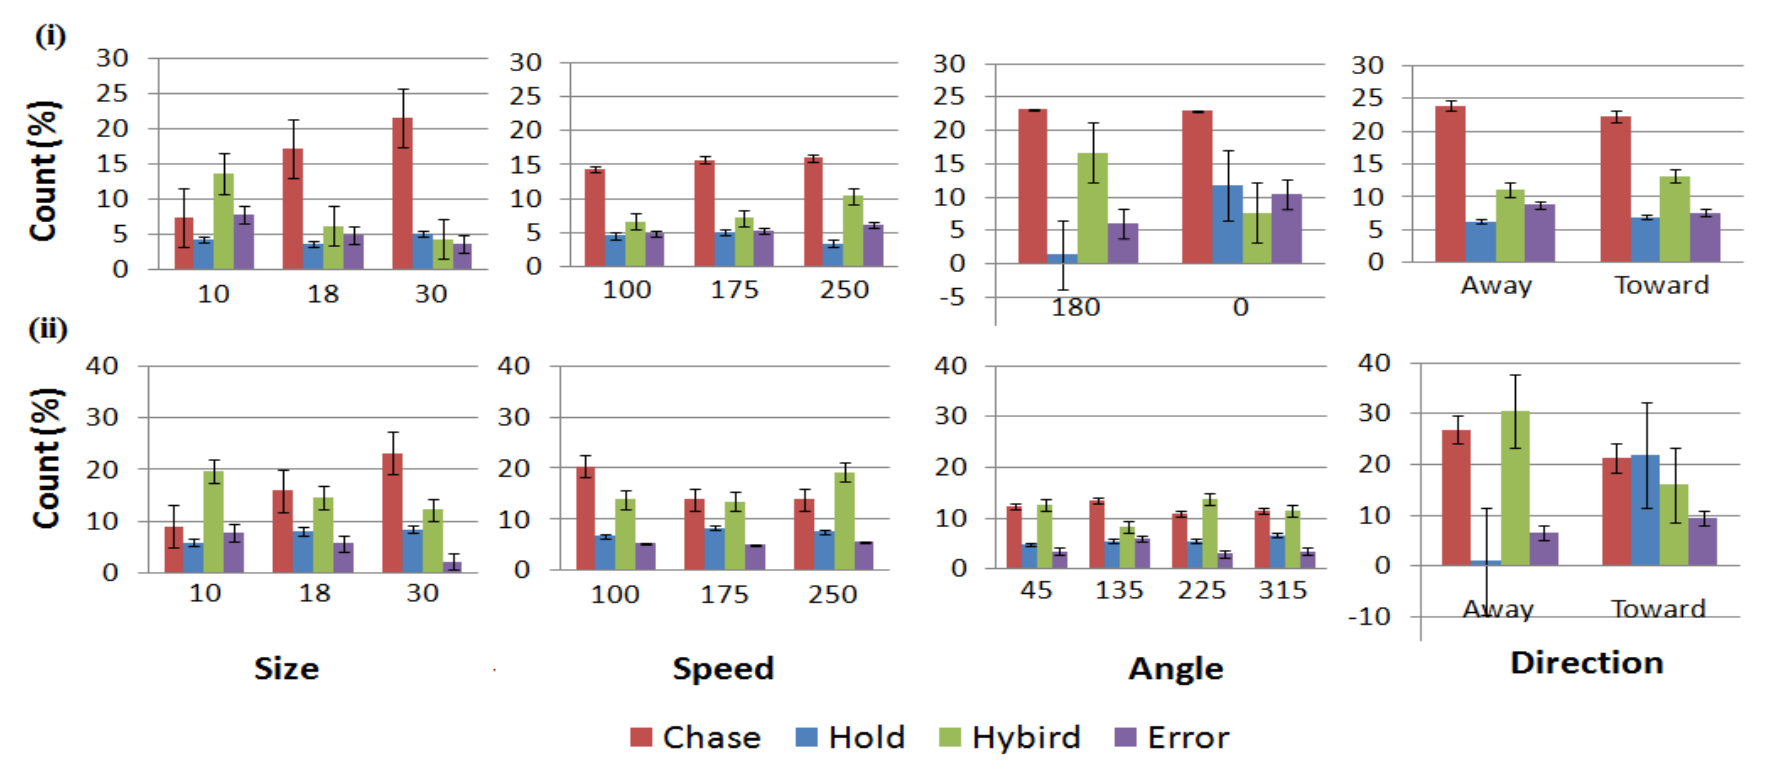
\includegraphics[width=\textwidth]{figures/ch2/holdTech}
		\caption[\emph{Hold} --- choix de la technique]{Les choix de technique faits par les sujets en fonction des paramètres de la cible --- sa taille, sa vitesse, sa direction et l'angle de sa direction. Les résultats de la première ligne de graphiques correspondent aux essais en 1D, et ceux de la seconde, en 2D. On constate que les cibles « faciles » tendent à inciter au choix de \emph{Chase}, que les sujets décrivent comme plus rapide, tandis que les cibles plus difficiles à sélectionner encouragent le choix de \emph{Hold} ou \emph{Hybrid}. La taille et la vitesse sont les paramètres dont l'effet est le plus significatif. Les barres notées \emph{Error} correspondent simplement aux essais ratés, c'est-à-dire ceux pour lesquels le sujet à délenché la sélection hors de la cible. Crédit : \cite{hajri2011moving}.}
		\label{fig:holdTech}
	\end{figure}
	
	La figure~\ref{fig:holdRatio} détaille la répartition entre l'utilisation de \emph{Chase} et \emph{Hold} dans une phase identifiée comme \emph{Hybrid}. Là encore, on constate que la difficultée est corrélée avec une utilisation accrue de la technique \emph{Hold.}
	
	\begin{figure}[H]
		\centering
		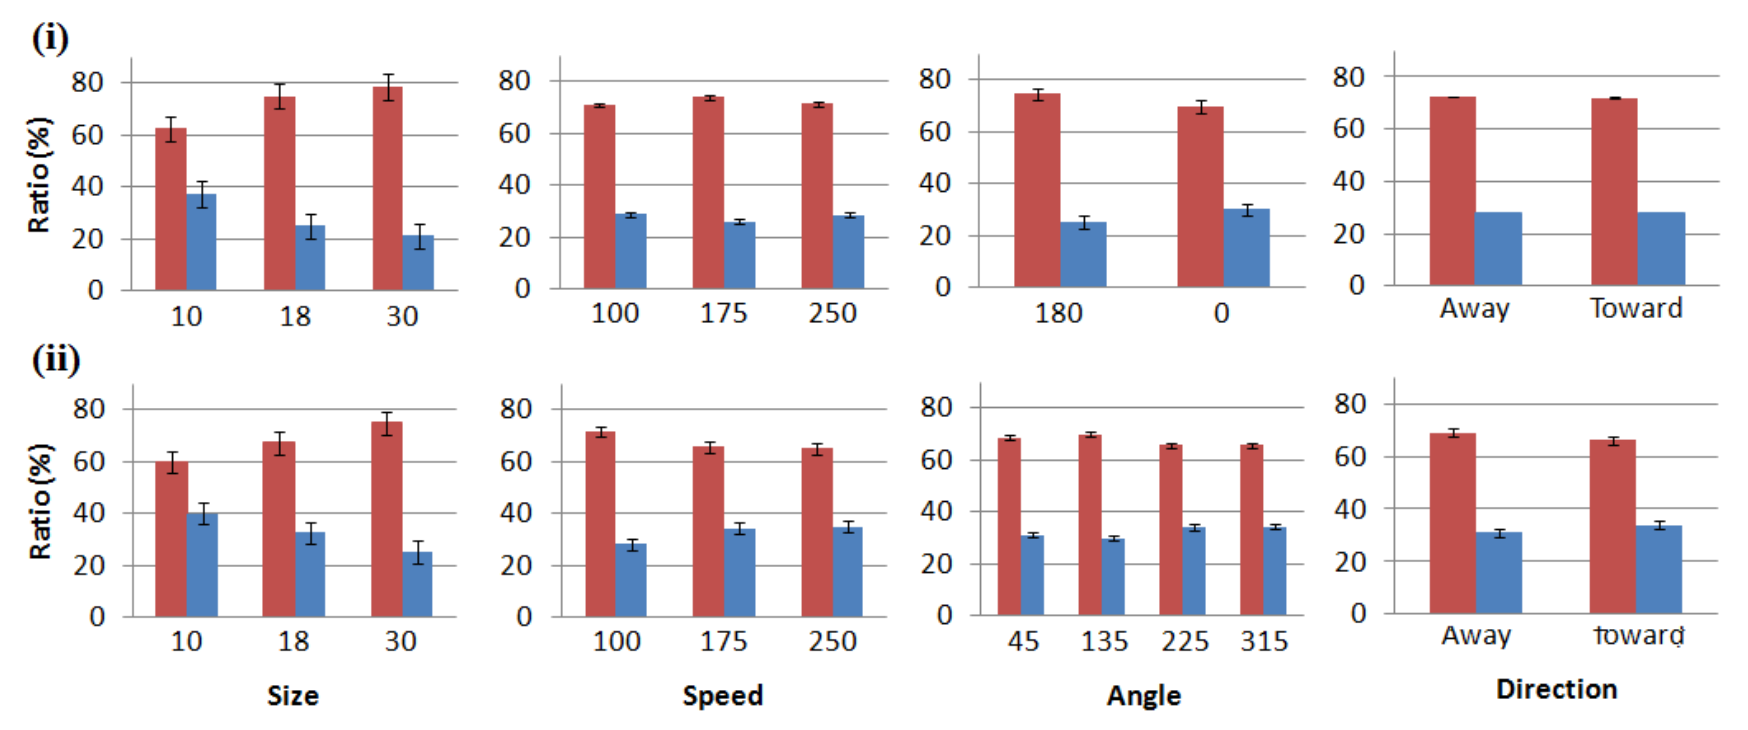
\includegraphics[width=\textwidth]{figures/ch2/holdRatio}
		\caption[\emph{Hold} --- répartition \emph{Hold/Chase} en mode \emph{Hybrid}]{épartition entre l'utilisation de \emph{Chase} et \emph{Hold} dans une phase identifiée comme \emph{Hybrid}. L'angle et la direction n'ont pas d'effet significatif mais la vitesse (à mesure qu'elle augmente) et la taille (à mesure qu'elle diminue) sont corrélées avec une utilisation accrue de la technique \emph{Hold}, malgré l'étape supplémentaire qu'elle implique. C'est résultats sont cohérents avec ceux observés hors du mode \emph{Hybrid}. Crédit : \cite{hajri2011moving}.}
		\label{fig:holdRatio}
	\end{figure}
	
	\subsection{Inconvénients}
	Néanmoins et bien qu'il soit atténué, le problème d'occultation demeure. Mais surtout, cette technique impose d'arrêter l'animation ou la simulation à la source des mouvements des cibles, ce qui est inacceptable dans bon nombre d'applications, comme la plupart des jeux vidéo, par exemple.
	
	Pour les simulations moléculaires ou encore le contrôle des espaces aérien, maritime, terrestre, les retransmissions d'événements sportifs, etc., cela implique une perte de connexion avec le réel, qui peut dans certains cas être inacceptable.
	
	Un cas particulier mérite d'être souligné : celui des simulations interactives collaboratives, c'est-à-dire impliquant plusieurs utilisateurs pouvant éventuellement être distants l'un de l'autre, et utiliser des dispositifs différents mais synchronisés. Dans un tel contexte, \emph{Hold} impliquerait soit l'imposition par un utilisateur à tous les autres d'un arrêt de la simulation, soit la désynchronisation des différentes simulations.
	
	Certains jeux vidéo sont également dans ce cas de figure, avec le facteur aggravant qu'ils peuvent impliquer un très grand nombre d'utilisateurs simultanés.
	
\section{\emph{raycasting}}
	\subsection{Principe et avantages}
	Le \emph{raycasting} est une technique de sélection conceptuellement très simple : un périphérique est utilisé pour lancer un rayon virtuel, généralement le long d'un axe du périphérique. Le rayon peut ensuite croiser un objet, ce qui permet de le sélectionner. Cette technique est parfois appelée \emph{laser gun}~\cite{liang1994jdcad}, et elle est illustrée par la figure~\ref{fig:dCanvas2}.
	
	Elle a plusieurs avantages : elle permet de sélectionner un objet à n'importe quelle distance, sans avoir à se déplacer ; on peut sélectionner un objet très éloigné de la position initiale du curseur sans avoir à faire de grand mouvement, puisqu'il suffit de changer l'orientation du périphérique de pointage, donc d'un simple mouvement de poignet.
	
	Cependant, pour les objets de petite taille apparente, la sélection peut être difficile, car elle requiert une précision angulaire élevée. De plus, si le système de \emph{tracking} qui fournit la position et l'orientation du périphérique de pointage produit un signal bruité, la difficulté de sélection s'en trouve encore accrue. Par conséquent, des techniques dérivées du \emph{raycasting} ont été développées.
	
	Classiquement, on utilisera une technique de cône de sélection, comme par exemple \emph{Spotlight}~\cite{liang1994jdcad}, illustrée par la figure~\ref{fig:spotlight}. Comme le nom l'indique, les techniques de ce typent remplacent le rayon de sélection par un cône dont le sommet est placé sur le périphérique de pointage.
	
	\begin{figure}[H]
		\centering
		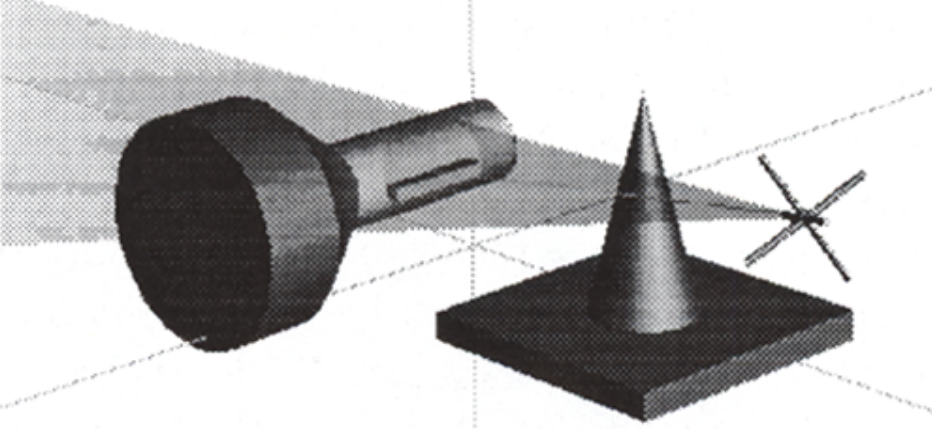
\includegraphics[width=\textwidth]{figures/ch2/spotlight}
		\caption[Cône de sélection : \emph{Spotlight}]{Illustration d'une technique de sélection par cône, baptisée \emph{Spotlight}. Les objets qui se trouvent dans le cône sont des candidats à la sélection : quand il y en a plusieurs, le plus proche de l'axe de révolution du cône est choisi ; en cas de proximité égale, le plus proche du périphérique de pointage est choisi. Crédit : \cite{liang1994jdcad}.}
		\label{fig:spotlight}
	\end{figure}
	
	Cela facilite la sélection, puisque les gestes n'ont plus besoin d'être aussi précis, mais peut ajouter de l'ambiguïté si deux objets se trouvent dans le cône de sélection. Le cas échéant, cette ambiguïté peut être levée de plusieurs façon, en fonction de la proximité à l'axe de révolution du cône, en fonction de la distance au périphérique de pointage, ou via une intervention directe de l'utilisateur.
	
	Le choix de l'angle du cône est important : plus il sera grand, plus la sélection sera facile mais potentiellement ambiguë ; plus il sera petit, plus la sélection sera difficile mais spécifique. Le choix de cet angle peut éventuellement être paramétrable, permettant à l'utilisateur de choisir ce qui lui convient le mieux, voire de l'ajuster à la volée en cours d'utilisation. Cet ajustement pourrait également être géré automatiquement par le système interactif, par exemple de façon analogue à ce qui est fait avec des pointeurs classiques dans le \emph{Bubble Cursor}~\cite{grossman2005bubble} ou \emph{DynaSpot}~\cite{chapuis2009dynaspot}.
	
	\subsection{Inconvénients}
	Lorsque l'environnement est particulièrement dense, la sélection par rayon ou cône devient difficile~\cite{kopper2011rapid}, car la précision requise devient très élevée, tant pour l'utilisateur que pour le système de suivi du périphérique de pointage. L'utilisation d'un cône facilite la sélection de petites cibles, mais ajoute un risque d'ambiguïté.
	
	Or, si diverses techniques peuvent aider à lever l'ambiguïté, leur utilisation est d'autant plus difficile que les cibles situées dans le volume du cône sont nombreuses, petites et\ldots{} mobiles. En effet, la mobilité des cibles nécessite d'effectuer des mouvements plus rapides pour les pointer, donc d'exercer plus de force, et de fait, d'être moins précis~\cite{schmidt1979motor}.
	
	Une solution à certains de ces problèmes peut être d'augmenter le ratio contrôle/affichage à proximité des cibles~\cite{frees2007prism, kopper2010human}, mais c'est au prix de l'introduction d'un décalage entre l'orientation réelle du périphérique de pointage et celle du rayon qu'il lance, ce qui peut être très troublant. En outre, cette solution pourrait être difficile à adapter aux cibles mobiles, surtout si elles sont rapides.
	
	Par conséquent, la sélection par rayon ou par cône ne saurait, à elle seule, être une option viable pour sélectionner de nombreuses et petites cibles~\cite{steed20043d}, \emph{a fortiori} si elles sont mobiles, rapides, et si leurs mouvements sont imprévisibles.
	
\section{\emph{Shadow Cone}}
	\subsection{Principe et avantages}
	~\cite{steed20043d}
	
	\subsection{Inconvénients}
	
	
\section{\emph{raycasting} avec disambiguïsation}
	Dans~\cite{grossman2006design}, Grossman \emph{et al.} proposent d'évaluer diverses techniques de sélection dérivées du \emph{raycasting} et ayant pour but de faciliter la désambiguïsation lorsque le rayon atteint plusieurs objets. Ces travaux sont présentés comme étant motivés par l'émergence d'écrans volumétriques~\cite{ebert1999realizing}, mais demeurent très pertinents pour des dispositifs d'affichage plus classiques, notamment stéréoscopiques.

	\subsection{\emph{Depth Ray}}
	\subsubsection{Principe}
	Le \emph{Depth Ray}~\cite{grossman2006design} fonctionne comme une technique de \emph{raycasting} traditionnelle, si ce n'est que la position du périphérique de pointage le long de son axe est prise en compte, comme le montre la figure~\ref{fig:depthRay}. Le rayon est augmenté d'un marqueur de profondeur que l'utilisateur déplace le long du rayon simplement en avançant ou en reculant le périphérique de pointage.
	
	\begin{figure}[H]
		\centering
		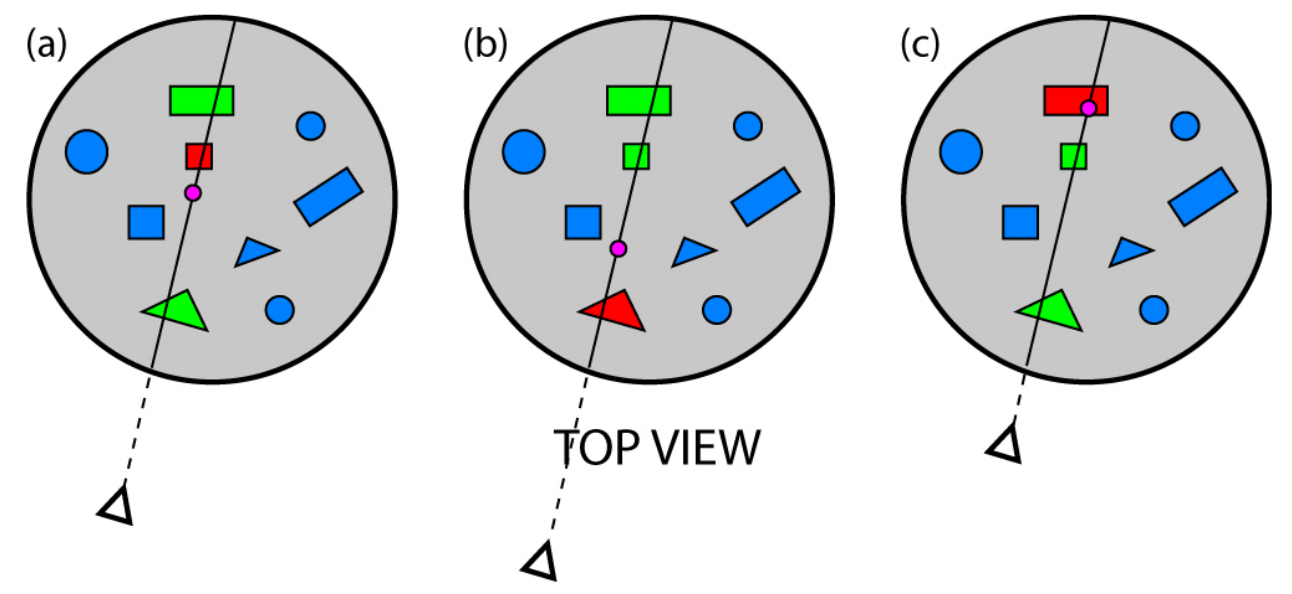
\includegraphics[width=\textwidth]{figures/ch2/depthRay}
		\caption[Principe du \emph{Depth Ray}]{Illustration du fonctionnement du \emph{Depth Ray}. (a) Un marqueur rose est utilisé pour sélectionner la cible intersectée la plus proche de lui --- notons que le marqueur fonctionne par proximité et n'a pas besoin d'être \emph{sur} la cible. (b) Reculer le périphérique de pointage recule le marqueur et permet de séletionner une cible plus proche. (c) Inversement, avancer le périphérique permet d'avancer le marqueur et de sélectionner une cible plus lointaine. Crédit : \cite{grossman2006design}.}
		\label{fig:depthRay}
	\end{figure}
	
	\subsection{\emph{Lock Ray}}
	\subsubsection{Principe}
	Le \emph{Lock Ray}~\cite{grossman2006design} fonctionne de la même façon que le \emph{Depth Ray}, si ce n'est qu'une fois que le rayon est positionné, il est \emph{verrouillé} --- d'où le nom --- afin de permettre à l'utilisateur de déplacer le marqueur de profondeur sans avoir à craindre de faire bouger le rayon par accident.
	
	\begin{figure}[H]
		\centering
		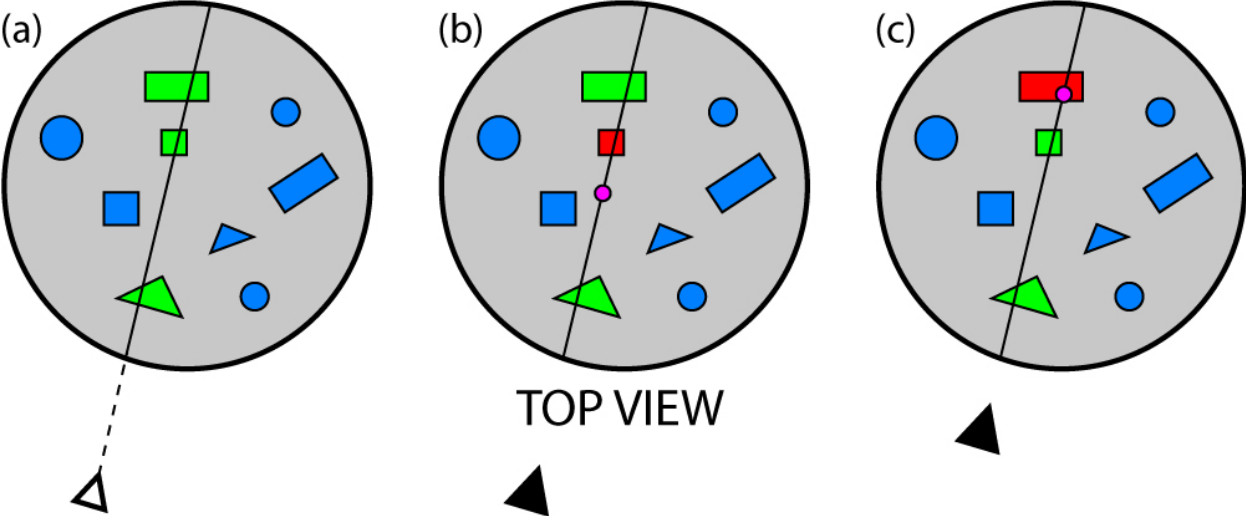
\includegraphics[width=\textwidth]{figures/ch2/lockRay}
		\caption[Principe du \emph{Lock Ray}]{Illustration du fonctionnement du \emph{Lock Ray}. (a) La sélection commence par une phase de \emph{raycasting} classique, sans marqueur de profondeur. (b) Une fois que l'utilisateur a pressé le bouton du périphérique un marqueur de profondeur apparaît au milieu du segmet du rayon inclus dans la sphère. (c) L'utilisateur peut déplacer le marqueur en déplaçant sa main, comme dans le \emph{Depth Ray}, et effectue la sélection en relâchant le bouton. Crédit : \cite{grossman2006design}.}
		\label{fig:lockRay}
	\end{figure}
	
	\subsection{\emph{Flower Ray}}
	\subsubsection{Principe}
	Comme le \emph{Lock Ray}, le \emph{Flower Ray}~\cite{grossman2006design} fonctionne avec deux phases distinctes. Dans la première, l'utilisateur place son rayon dans la position et l'orientation qu'il désire ; puis, il le fixe, et les objets croisés par le rayon « s'épanouissent » --- tout autour d'un curseur ponctuel, comme les pétales d'une fleur autour de son pistil, ainsi que l'illustre la figure~\ref{fig:flowerRay}. Dans le menu « floral » les objets sont disposés par ordre de profondeur croissante dans le sens horaire, avec le plus proche en haut à droite.
	
	\begin{figure}[H]
		\centering
		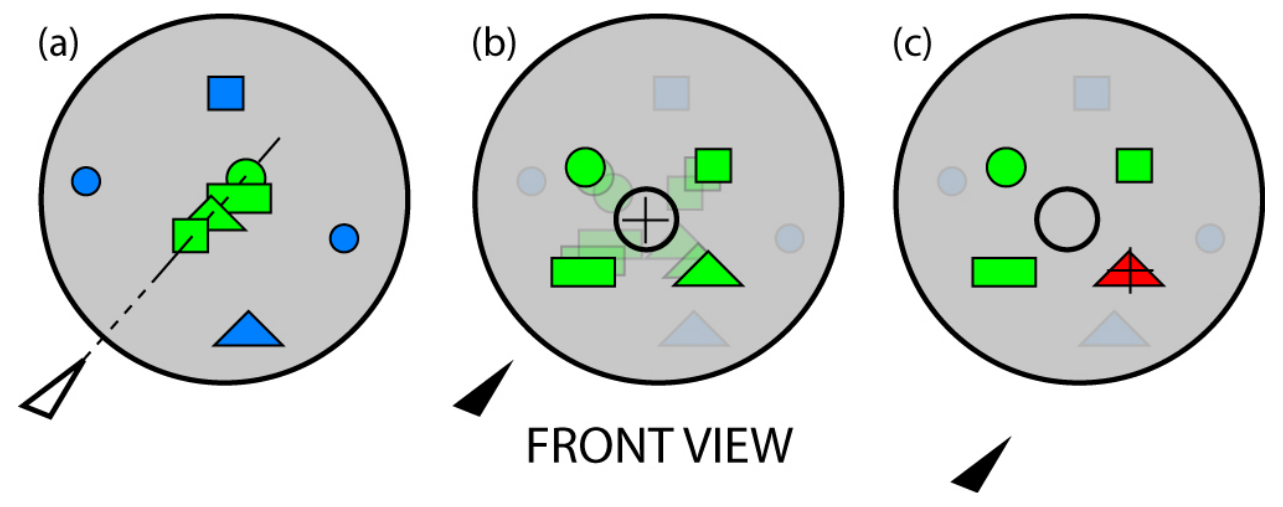
\includegraphics[width=\textwidth]{figures/ch2/flowerRay}
		\caption[Principe du \emph{Flower Ray}]{Illustration du fonctionnement du \emph{Depth Ray}. (a) Toutes les cibles croisées par le rayon sont colorées en vert. (b) Quand l'utilisateur presse le bouton de son périphérique, ces objets s'épanouissent en un menu de sélection autour d'un curseur poncuel, qui apparaît à cet instant. (c) L'utilisateur peut à présent pointer près de la cible et relâcher le bouton pour la sélectionner. Crédit : \cite{grossman2006design}.}
		\label{fig:flowerRay}
	\end{figure}
	
	\subsection{\emph{Smart Ray}}
	\subsubsection{Principe}
	Par définition, un rayon contient une infinité de points. Toutefois, si deux sont sécants, alors ils n'ont qu'un seul point en commun. Il donc possible d'utilier deux rayons pour effectuer une sélection par \emph{raycasting} sans aucune ambiguïté. Toutefois, cela nécessite deux périphériques de saisie et cela occupe les deux mains de l'utilisateur.
	
	Le \emph{Smart Ray}~\cite{grossman2006design} propose donc de faire cela avec deux rayons issus du même périphérique, mais mesurés à deux instant différents, selon une idée exposée mais non évaluée par Anthony Steed~\cite{steed2006towards}. Chaque objet se voit attribuer un « poids » qui croît d'autant plus que le rayon est proche de son centre, ou décroît d'autant plus qu'il en est loin, continuellement. L'objet dont le poids est le plus élevé peut être sélectionné, comme l'illustre la figure~\ref{fig:smartRay}.
	
	\begin{figure}[H]
		\centering
		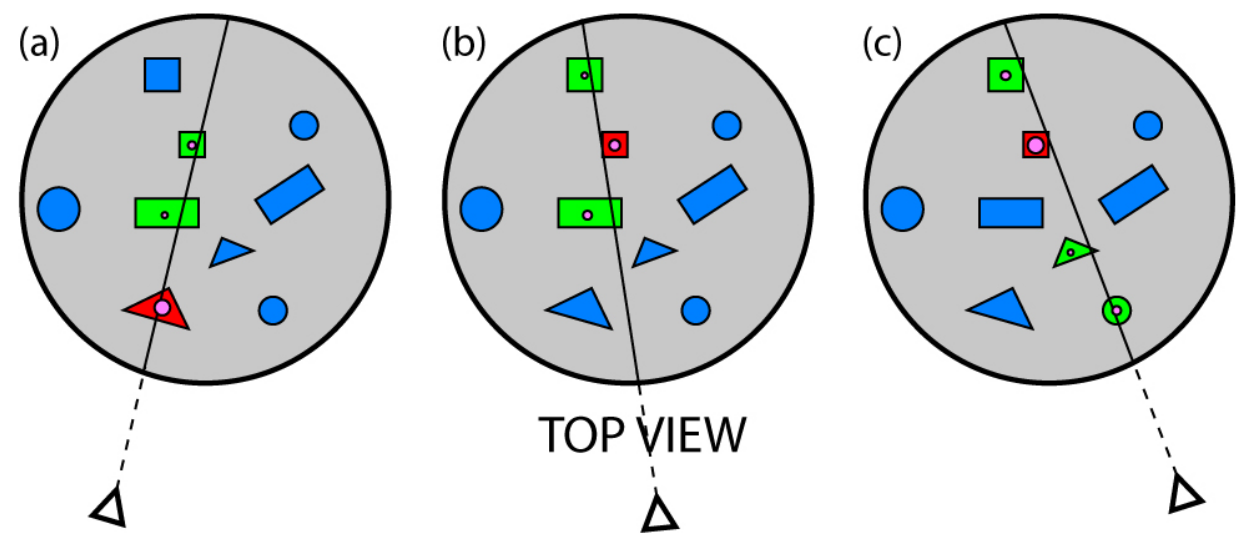
\includegraphics[width=\textwidth]{figures/ch2/smartRay}
		\caption[Principe du \emph{Smart Ray}]{Utilisation du \emph{Smart Ray} pour sélectionner le petit carré. (a) Les poids des cibles sont basés sur la distance entre le rayon et la cible, et visualisés par de petites sphères au centre de chaque cible. À tout moment, la cible avec le plus gros poids peut être sélectionnée. (b,c) Le rayon peut être repositionné en continu pour augmenter le poids de la cible visée, même si elle est occultée. Crédit : \cite{grossman2006design}.}
		\label{fig:smartRay}
	\end{figure}
	
	\subsection{Motivations}
	Grossman \emph{et al.}~\cite{grossman2006design} notent que les techniques présentées ci-dessus ont chacune des avantages et des inconvénients. Le \emph{Depth Ray} unifie les phases de sélection et de désambiguïsation, ce qui peut faire gagner du temps mais aussi causer des perturbations entre les phases. Le \emph{Lock Ray} sépare les phases explicitement, mais désambiguïse avec un menu linéaire. Le \emph{Flower Ray} propose un menu radial, théoriquement plus rapide, mais les utilisateurs doivent suivre l'animation pour ne pas perdre leur cible entre les deux phases. Enfin, le \emph{Smart Ray} fournit un mode de désambiguïsation implicite et possiblement plus fluide, mais potentiellement source de frustration s'il échoue à prédire correctement l'intention de l'utilisateur, comme toujours avec les techniques prédictives.
	
	\subsection{Évaluations}
	Avec ces mérites respectifs en tête, Grossman \emph{et al.} ont évalué ces quatre techniques dans un environnement dense, afin de rendre la désambiguïsation absolument nécessaire. De fait, la sélection par \emph{raycasting} classique est impossible, et donc ne fut pas évaluée ici. La technique de base considérée est donc le curseur ponctuel.

\section{Sélection en cascade, grossière, puis fine}
	\subsection{Principe général et avantages}
	Les techniques de cette catégorie divisent la sélection en deux phases (ou plus). Premièrement, une portion de l'espace visuel est sélectionnée. Cette première phase étant grossière, elle n'a pas besoin d'être précise, et peut être très rapide. Par exemple, avec un simple périphérique de pointage, tel qu'une souris, un ratio contrôle/affichage (\emph{control/display, C/D}) très faible peut être utilisé. Le curseur (ou autre medium de sélection) peut ainsi se placer très rapidement sur la zone d'intérêt, mais n'a pas besoin d'être précisément sur la cible pour délencher la deuxième phase : la sélection (plus) fine. Dans celle-ci, l'utilisateur sélectionne la cible elle-même, par exemple à l'aide d'un ratio C/D plus élevé, ou bien affine encore l'espace de sélection, jusqu'à ce qu'une phase finale permette la sélection effective de la cible.
	 
	Du point de vue de la loi de Fitts, au cours d'une phase grossière, la cible bénéficie d'une largeur accrue (car c'est toute une zone autour de la cible qui est visée) tandis que la phase finale offre une distance réduite, puisque le curseur se trouve déjà près de la cible. Quoiqu'il y ait probablement un certain « coût cognitif » lié au basculement d'une phase à l'autre, et en tout cas un coût temporel associé à la pression d'un bouton ou à toute autre action permettant de passer à la phase suivante, les techniques de sélection en cascade peuvent améliorer significativement les performances de sélection, même pour les tâches dont l'indice de difficulté est élevé~\cite{kopper2011rapid}.
	
	La sélection en cascade revient, en substance, à préférer une série de tâches très rapides et faciles à une seule tâche nécessitant une précision élevée, prenant du temps et pouvant être source d'erreur plus ou moins fréquentes. Observons que la sélection en cascade, du fait de la réduction du taux d'erreur qu'elle permet, présente un intérêt particulier pour les tâches critiques, celles pour lesquelles une erreur peut avoir des conséquences graves.
	
	\subsubsection{\emph{Sphere-casting refined by QUAD-menu
(SQUAD)}}
	\paragraph{Principe et avantages.}	 
	Un exemple typique de méthode de sélection en cascade est la technique \emph{Sphere-casting refined by QUAD-menu
(SQUAD)}~\cite{kopper2011rapid}. Avec SQUAD, l'utilisateur commence par sélectionner un volume contenant sa cible ; puis, il affine progressivement sa sélection en choisissant le sous-ensemble de cibles contenant celle qu'il veut, via un menu à quatre options affichant tous les objets n'ayant pas encore été éliminés ; \emph{in fine}, le dernier objet restant est sélectionné. Aucune des sous-tâches de SQUAD ne nécessite d'être précis. Le fonctionnement de cette technique est illustré par la figure~\ref{fig:squad}.

	\begin{figure}[H]
		\centering
		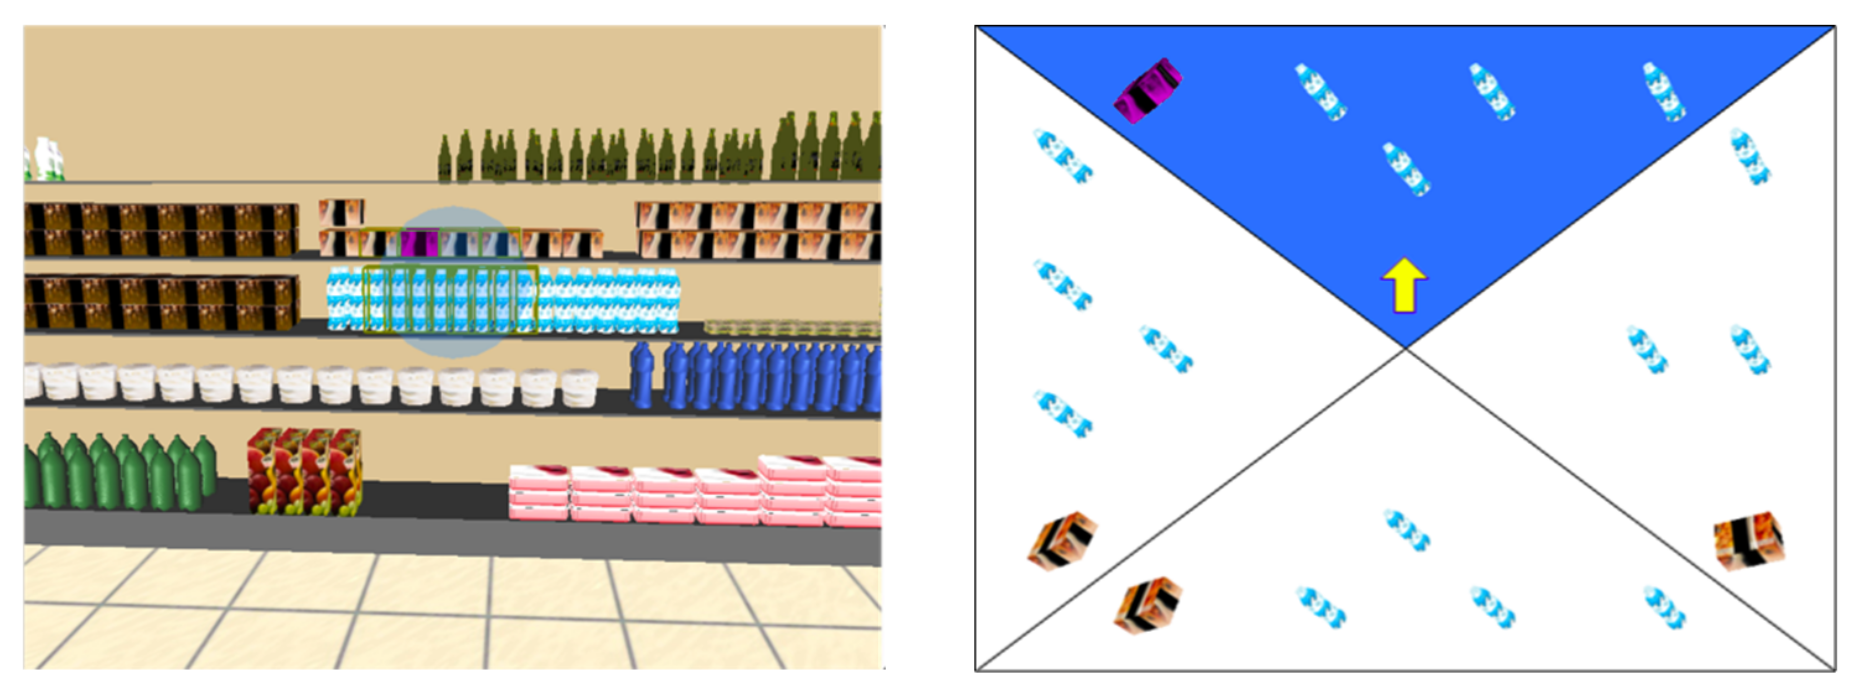
\includegraphics[width=\textwidth]{figures/ch2/squad}
		\caption[Fonctionnement de la technique SQUAD]{La technique SQUAD. À gauche, la première étape de sélection, au cours de laquelle l'utilisateur présélectionne une portion de l'espace à l'aide d'une sphère. À droite, la phase suivante, permettant d'affiner la sélection. Les objets présélectionnés avec la sphère sont uniformément répartis dans quatre quadrants d'un menu, et l'utilisateur n'a plus qu'à choisir le quadrant contenant l'objet qu'il souhaite sélectionner. Les autres quadrants se vident, puis les objets du quadrant sélectionné sont répartis dans les quatre afin de permettre, dans une nouvelle étape, d'affiner encore la sélection. L'opération est répétée jusqu'à ce qu'il n'y ait plus qu'un objet, qui est sélectionné. Crédit : \cite{kopper2011rapid}.}
		\label{fig:squad}
	\end{figure}
	
	Bien que le procédé puisse paraître pénible, il permet d'affiner la sélection jusqu'au dernier élément en $log_{4}(n)$ étapes, où $n$ est le nombre d'objets présélectionnés par la sphère au cours de la première étape. Naturellement, il faut ajouter à cela l'étape de présélection. Au total, la sélection d'un objet parmi 256 se fait en seulement 5 étapes, où chaque étape peut être très rapide.
	
	En pratique, dans~\cite{kopper2011rapid}, SQUAD fut évaluée avec des objets uniformes : des sphères de rayons identiques. Seule la couleur variait, avec du gris pour des distracteurs et du rouge pour la cible à sélectionner, comme on le voit sur la figure~\ref{fig:squad2}. 
	
	\begin{figure}[H]
		\centering
		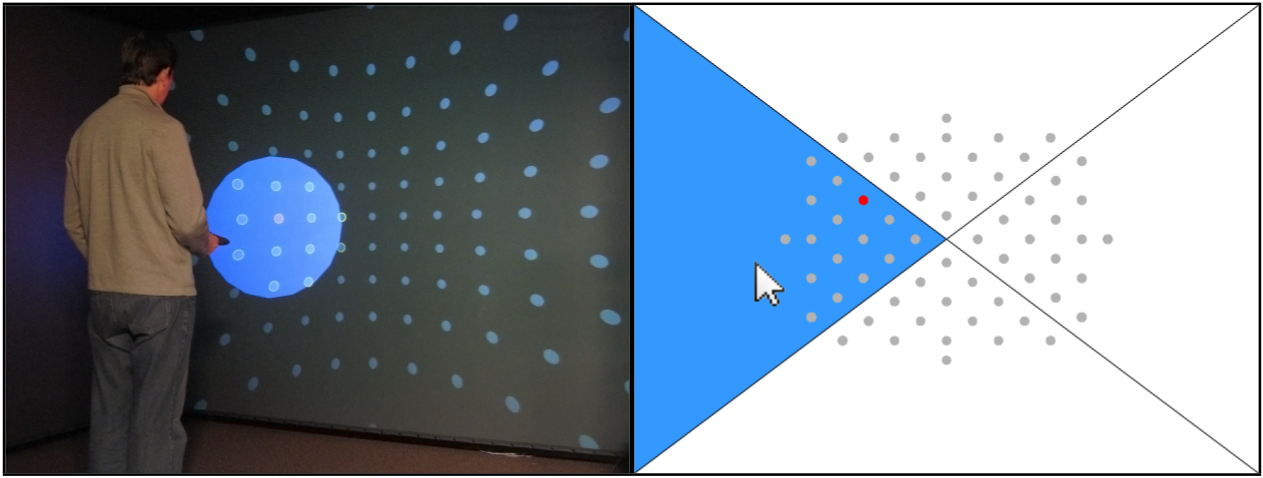
\includegraphics[width=\textwidth]{figures/ch2/squad2}
		\caption[La technique SQUAD --- évaluation]{La technique SQUAD telle qu'elle fut évaluée dans~\cite{kopper2011rapid}. Dans la première phase (à gauche) les petites sphères sont réparties sur la surface d'une grande sphère invisible centrée sur l'utilisateur, de sorte qu'elles sont toutes à la même distance de lui, afin qu'elles aient toutes une taille apparente égale une fois projetées sur l'écran. La cible à saisir est identifiée par sa couleur rouge, ce qui la rend facile à repérer, notamment dans la seconde phase, à droite. Seule l'orientation du périphérique de pointage était prise en compte dans la première phase, et les sujets avaient pour consigne de maintenir la sa position dans une zone déterminée. Crédit : \cite{kopper2011rapid}.}
		\label{fig:squad2}
	\end{figure}
	
	\paragraph{Performances.}
	Les performances de SQUAD, comparée au \emph{raycasting} et en fonction du nombre de distracteurs sont détaillées sur la figure~\ref{fig:squadDensity}. On constate que SQUAD offre de meilleures performances en environnement dense, de moins bonnes en environnement peu dense, et des résultats comparables entre les deux. Les mêmes résultats sont présentés sur la figure~\ref{fig:squadSize}, mais en fonction de la taille des cibles. Comme attendu, les performances de SQUAD sont à peu près constantes tandis que le \emph{raycasting} est d'autant plus performant que les cibles sont grandes. De fait, la technique SQUAD est avantageuse avec de petites cibles, désavantageuses quand elles sont grandes, et à peu près équivalent entre les deux.
	
	\begin{figure}[ht]
		\centering
		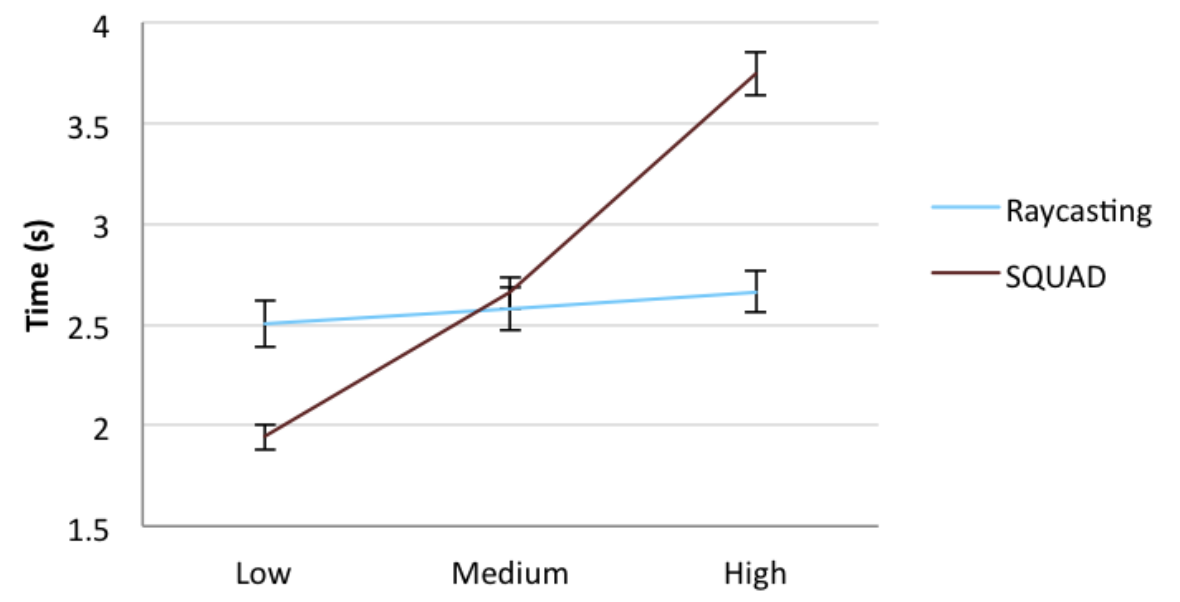
\includegraphics[width=\textwidth]{figures/ch2/squadDensity}
		\caption[SQUAD --- Résultats : densité]{Performances de la technique SQUAD en fonction de la densité de distracteurs, comparées avec celle du \emph{raycasting} classique. Les performances de cette dernière technique ne sont pas significativement modifiées par la densité, même si une légère corrélation est visible, potentiellement expliquée par l'augmentation du temps de recherche visuelle pour trouver la cible. C'est assez logique car l'indice de difficulté n'est pas modifié par la densité de distracteurs, seul le temps de réaction peut l'être. En revanche, les performances de SQUAD sont fortement affectées, ce qui là encore est logique puisque le nombre d'étapes dans la seconde phase en dépend directement. En pratique, SQUAD brille particulièrement dans les conditions de faible densité, mais se montre désavantageuse quand les distracteurs sont nombreux. Crédit : \cite{kopper2011rapid}.}
		\label{fig:squadDensity}
	\end{figure}
	
	\begin{figure}[ht]
		\centering
		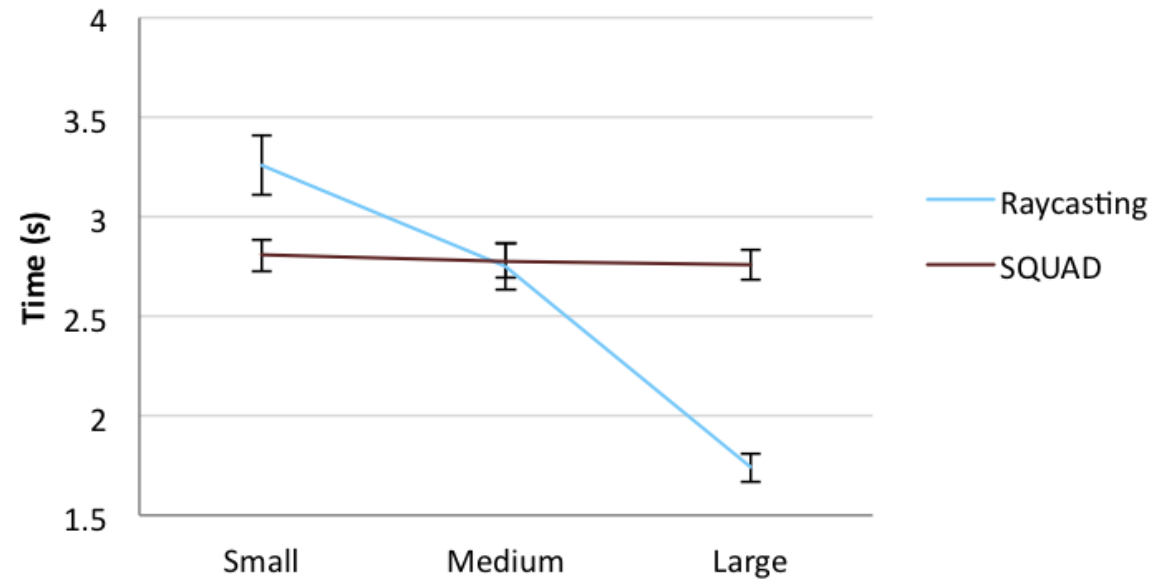
\includegraphics[width=\textwidth]{figures/ch2/squadSize}
		\caption[SQUAD --- Résultats : récapitulatif]{Performances de la technique SQUAD comparées avec celle du \emph{raycasting} classique, en fonction de la taille des cibles, et pour différentes densités de distracteurs. Notez que les performances du \emph{raycasting} sont une moyenne de ses performances sur toutes les densités, puisqu'elles n'en dépendent pas. La technique SQUAD se montre clairement plus performante à faible densité, mais se montre capable de gérer de très petites cibles sans augmentation notable du temps de sélection, ce qui est très intéressant pour certaines applications. Pour les cas les plus faciles avec de grosses cibles, on préférera le \emph{raycasting}, en particulier dans ses formes améliorées. Crédit : \cite{kopper2011rapid}.}
		\label{fig:squadSize}
	\end{figure}
	
	Un récapitulatif de ces résultats est présenté sur la figure~\ref{fig:squadRecap}. On constate que la technique SQUAD gère très bien les petites cibles, mais voit ses performances chuter avec le nombre de distracteurs. Notons par ailleurs que le taux d'erreurs avec SQUAD était extrêmement faible, avec seulement 0,7~\%{}, ce qui est un atout notable pour cette technique. De fait, si l'on considérait non pas les temps de sélection, mais les temps de sélection normalisés par rapport aux erreurs, l'évaluation serait nettement plus favorable à SQUAD.
	
	\begin{figure}[ht]
		\centering
		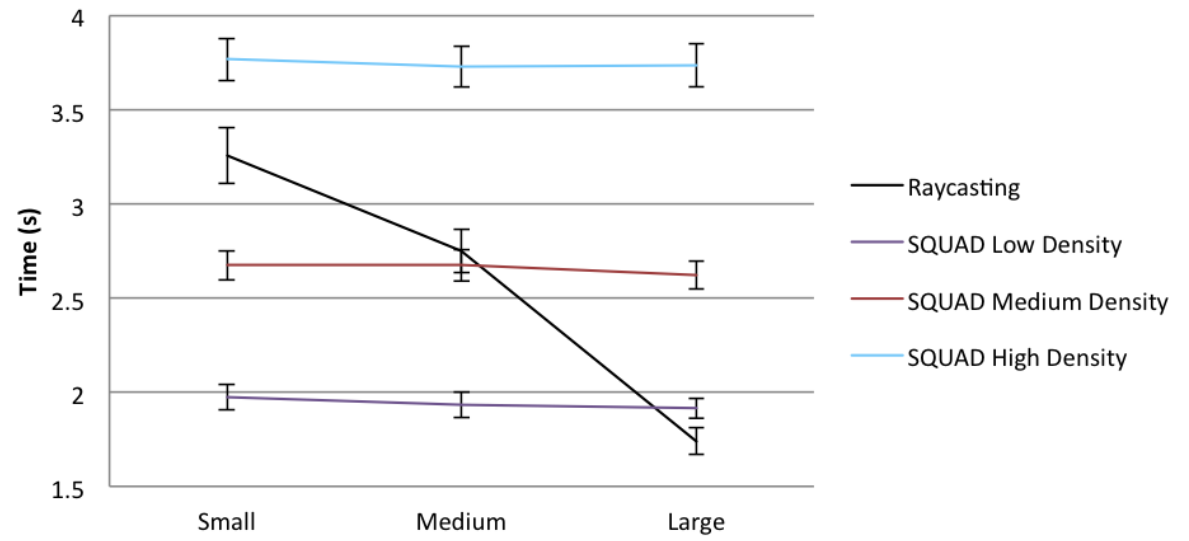
\includegraphics[width=\textwidth]{figures/ch2/squadRecap}
		\caption[SQUAD --- Résultats : taille]{Performances de la technique SQUAD en fonction de la taille de la cible, comparées avec celle du \emph{raycasting} classique. Les performances de SQUAD ne sont pas significativement modifiées par la taille, même si une légère corrélation négative est visible, potentiellement expliquée par l'augmentation du temps de recherche visuelle pour trouver la cible quand elle est petite. C'est assez logique car l'indice de difficulté n'est pas modifié par la taille de la cible, puisque seul le quadrant qui la contient doit être sélectionné, mais le temps de réaction peut l'être. En revanche, les performances du \emph{raycasting} sont fortement affectées, ce qui là encore est logique puisqu'une petite cible a un indice de difficulté bien plus élevé. En pratique, SQUAD brille particulièrement avec de petites cibles, mais se montre désavantageuse quand elles sont grandes. Crédit : \cite{kopper2011rapid}.}
		\label{fig:squadRecap}
	\end{figure}
	
	\paragraph{Inconvénients.}
	La chute des performances de SQUAD en cas de forte densité de distracteurs est certes un inconvénient de la technique, mais ce n'est peut-être pas le principal. En effet, au cours de la seconde phase, les objets sont répartis uniformément et aléatoirement dans quatre quadrants, pour que l'utilisateur sélectionne le bon. Celui-ci doit donc être capable de l'identifier visuellement le plus rapidement possible.
	
	Or, dans certains cas de figure, la cible n'est pas intrinsèquement différente des distracteurs, mais est choisie en fonction de sa position dans l'espace, par exemple. C'est notamment le cas le plus fréquent pour des simulations moléculaires, dans lesquels l'utilisateur peut vouloir sélectionner un atome d'un certain type (par exemple du carbone) parce qu'il se situe à un endroit spécifique, au sein d'une structure spécifique. Si tous les atomes étaient répartis dans des quadrants, il deviendrait impossible de distinguer cet atome de carbone des milliers d'autres.
	
	De plus, la technique SQUAD telle qu'elle existe fait l'hypothèse de cibles statiques, ce qui n'est pas le cas dans les applications qui nous intéressent. Certes, des cibles mobiles pourraient le rester dans leur quadrant, mais ce mouvement serait hors contexte et il est douteux qu'il puisse conserver du sens ou transmettre une information de valeur à l'utilisateur.
	
	Il nous apparaît donc que la technique SQUAD ne peut fournir de résultats satisfaisants qu'avec de petites cibles statiques dans des environnements de densité modérée, et à condition que la cible soit très distincte des distracteurs, suffisamment pour pouvoir être identifiée visuellement le plus rapidement possible.
	
	\subsubsection{\emph{Disambiguation Canvas}}
	\paragraph{Principe et avantages.}
	La technique du \emph{Disambiguation Canvas}~\cite{debarba2013disambiguation} est un autre exemple de technique de sélection en cascade, et est illustrée par la figure~\ref{fig:dCanvas}.
		 
	\begin{figure}[H]
		\centering
		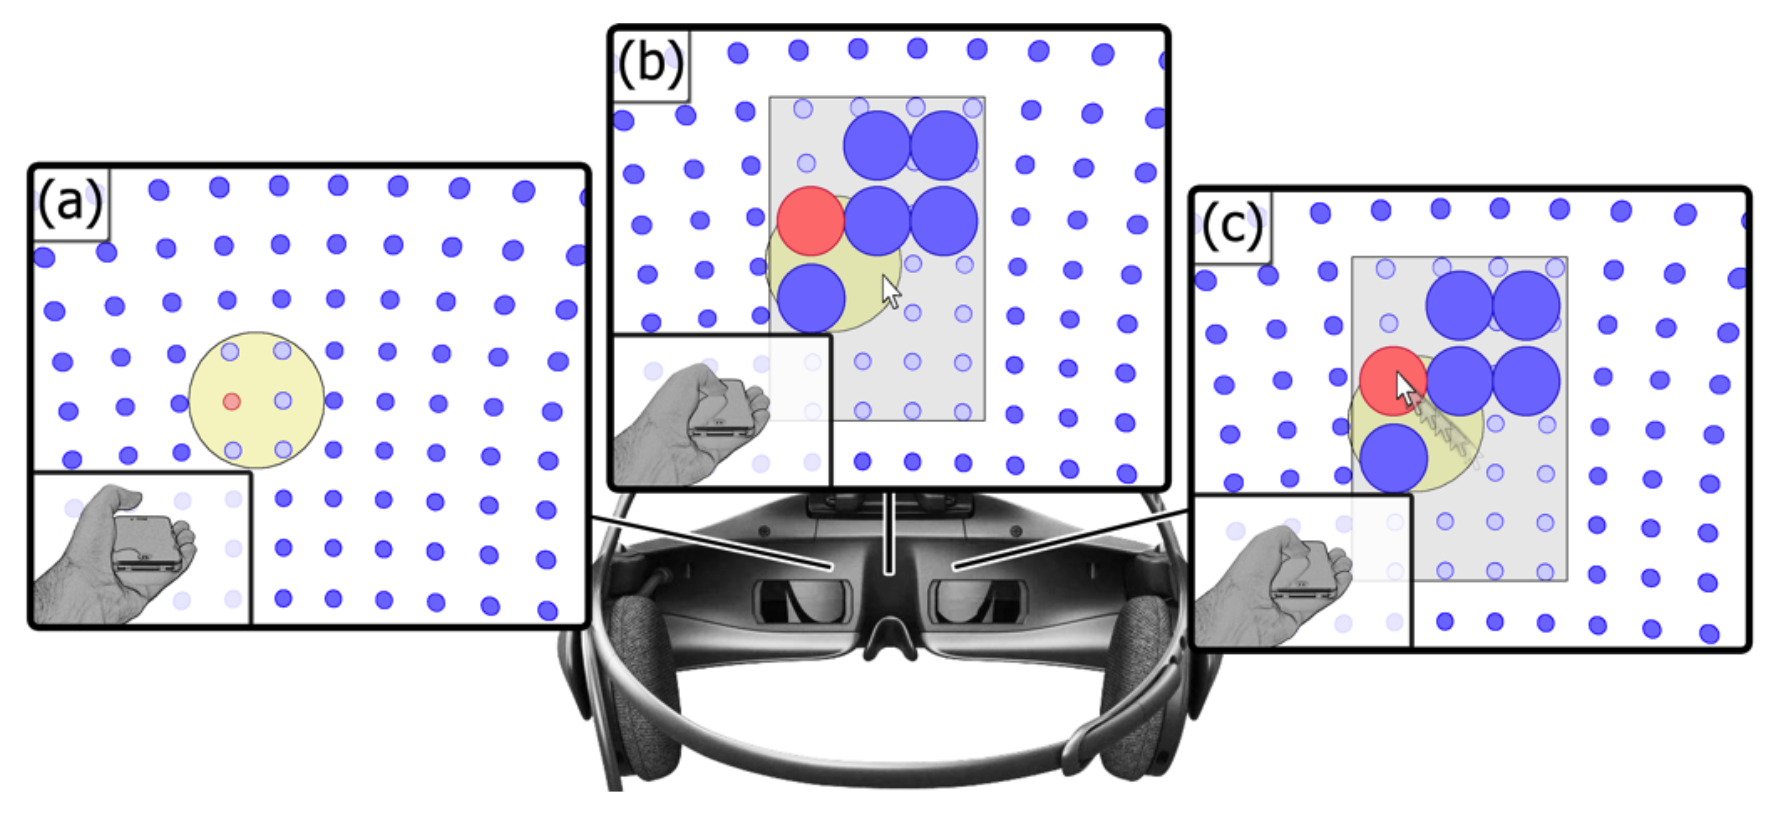
\includegraphics[width=\textwidth]{figures/ch2/dCanvas}
		\caption[\emph{Disambiguation Canvas}]{Fonctionnement du \emph{Disambiguation Canvas}, une technique de sélection en cascade. (a) : L'utilisateur pointe vers la région de l'espace où l'objet de son intérêt est situé ; cette présélection se fait par \emph{volume casting}, c'est-à-dire que le périphérique de pointage contrôle un volume de sélection dans l'espace virtuel. (b) : Une fois la présélection faite, une « toile » (\emph{canvas}) de sélection (c'est-à-dire un rectangle partiellement transparent) s'ouvre et les cibles présélectionnées y sont disposées après avoir été agrandies. La toile de sélection correspond à un \emph{mapping} absolu de l'écran tactile d'un périphérique de saisie (un \emph{smartphone}, en l'occurrence, mais cela pourrait être une tablette) ce qui permet à l'utilisateur de sélectionner l'objet désiré avec son pouce. Notez que cette technique est compatible avec les HMD et qu'elle n'affiche pas le petit encadré représentant la main de l'utilisateur en bas à gauche de chaque image ; ces encadrés sont présents ici à des fins purement illustratives. Crédit : \cite{debarba2013disambiguation}.}
		\label{fig:dCanvas}
	\end{figure}
	
	La figure~\ref{fig:dCanvas2} fournit une illustration supplémentaire et peut-être un peu plus claire de cette technique. Elle a pour avantage de ne nécessiter qu'un \emph{smartphone} comme périphérique de pointage pour la phase grossière, et de le réutiliser pour la sélection finale dans la phase fine. Dans la première, il est utilisé pour faire une présélection à l'aide d'une sphère, comme dans SQUAD~\cite{kopper2011rapid} ; dans la seconde, les objets présélectionnés sont arrangés dans un rectangle de même ratio d'aspect que l'écran du téléphone, et l'utilisateur n'a plus qu'à appuyer avec son pouce sur la zone de l'écran du téléphone correspondant à la zone du rectangle de sélection où se trouve la cible (se rapporter à la figure~\ref{fig:dCanvas} pour plus de clarté).
	
	\begin{figure}[H]
		\centering
		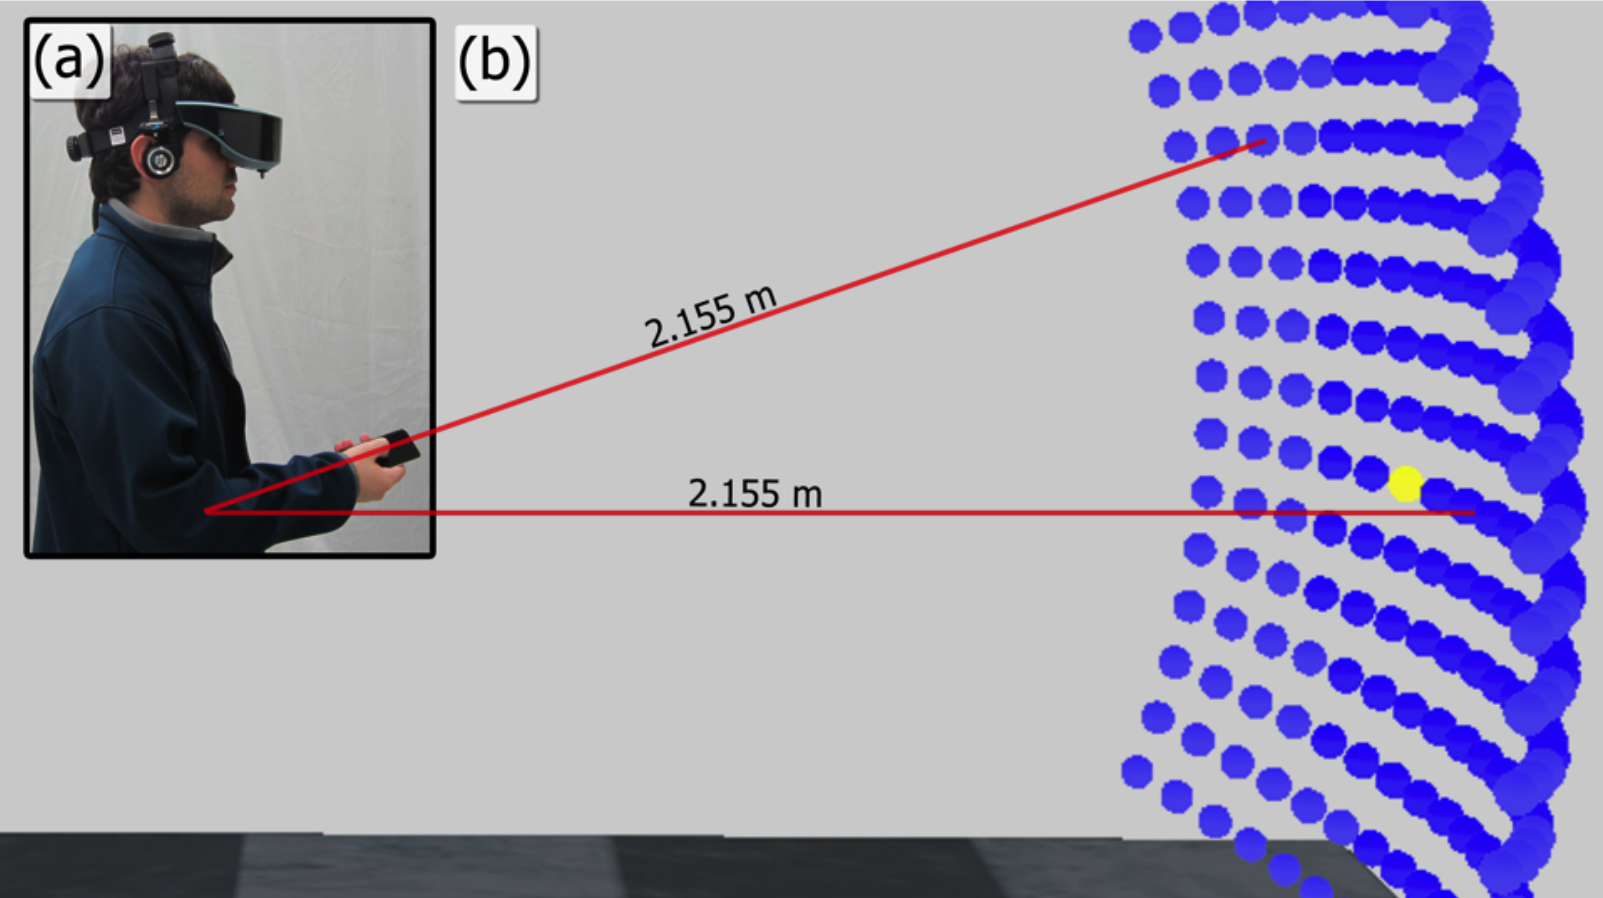
\includegraphics[width=\textwidth]{figures/ch2/dCanvas2}
		\caption[\emph{Disambiguation Canvas}, bis]{Fonctionnement du \emph{Disambiguation Canvas}. En (a), une photo d'un utilisateur de la technique, équipé d'un HMD et d'un pointeur ; en (b), l'espace virtuel utilisé pour évaluer la technique. Comme dans l'évaluation originale de SQUAD, les petites sphères sont réparties sur la surface d'une grande sphère invisible~\cite{kopper2011rapid}, ce qui permet d'uniformiser leurs tailles apparentes. Crédit : \cite{debarba2013disambiguation}.}
		\label{fig:dCanvas2}
	\end{figure}
	
	Pour définir un agencement optimal des objets dans la deuxième phase, dite de désambiguïsation, Debarba \emph{et al.} ont opté pour une étape de calibrage présentée sur la figure~\ref{fig:dCanvasLayout}.
	
	\begin{figure}[ht]
		\centering
		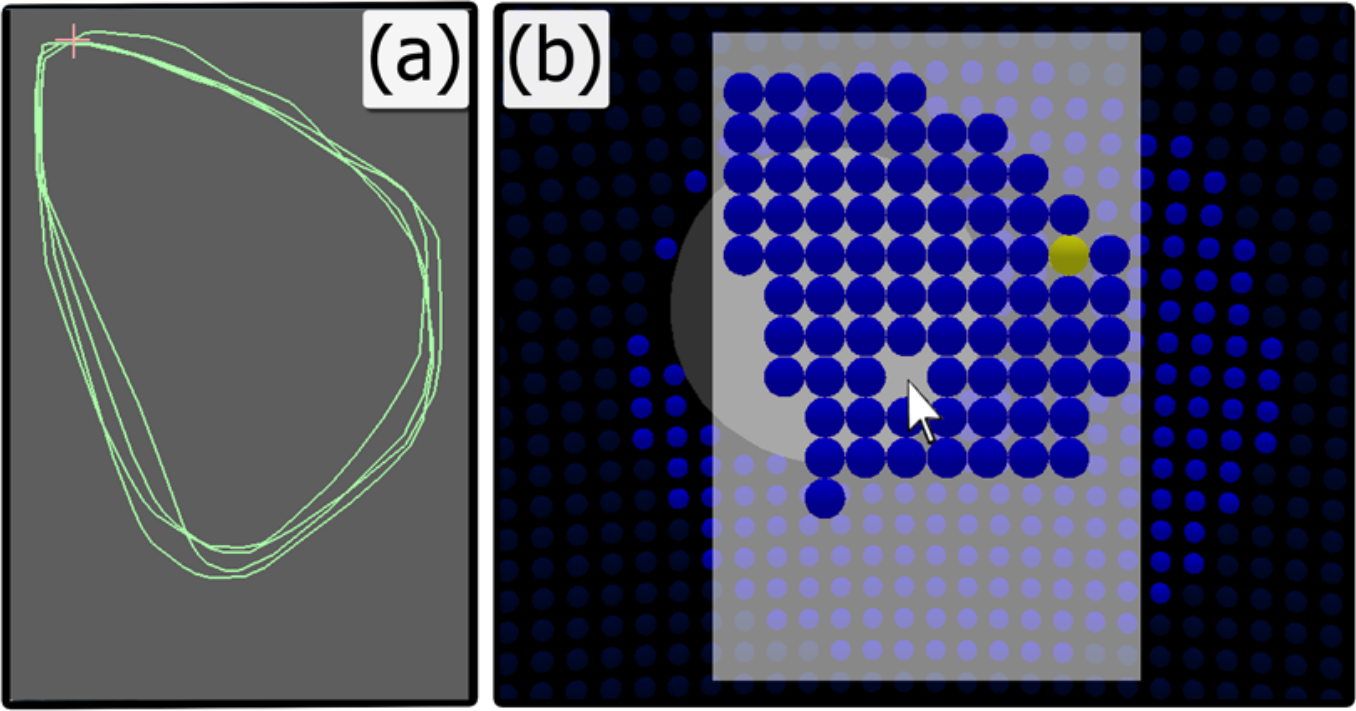
\includegraphics[width=\textwidth]{figures/ch2/dCanvasLayout}
		\caption[\emph{Disambiguation Canvas} --- Calibrage]{En (a), une étape de calibrage pour la deuxième phase du \emph{Disambiguation Canvas}. On demande ici à l'utilisateur de faire le tour de l'écran avec son pouce, en essayant de s'approcher des bords. Il en résulte un motif fermé représentant l'espace que l'utilisateur peut atteindre confortablement. En (b), cet espace est utilisé pour répartir les objets parmi lesquels figure la cible, que l'utilisateur pourra donc sélectionner aisément. Par défaut, l'emplacement où se trouve le curseur est laissé vide, pour éviter les sélections accidentelles et pour faciliter l'annulation en cas d'erreur au cours de la première phase. Crédit : \cite{debarba2013disambiguation}.}
		\label{fig:dCanvasLayout}
	\end{figure}
	
	Notez que les objets présélectionnés sont aggrandis ou rapetissés pour emplir l'espace de sélection dans la seconde phase. De fait, leur taille dans cette phase dépend essentiellement du nombre d'objets préselectionnés dans la première, plus que de la taille des objets eux-mêmes. De fait, la difficulté effective de sélection des objets dépend plus du nombre d'objets présélectionnés (donc indirectement de la densité de distracteurs) que de la taille réelle de l'objet visé, comme le montre la figure~\ref{fig:dCanvasDensity}.
	
	\begin{figure}[ht]
		\centering
		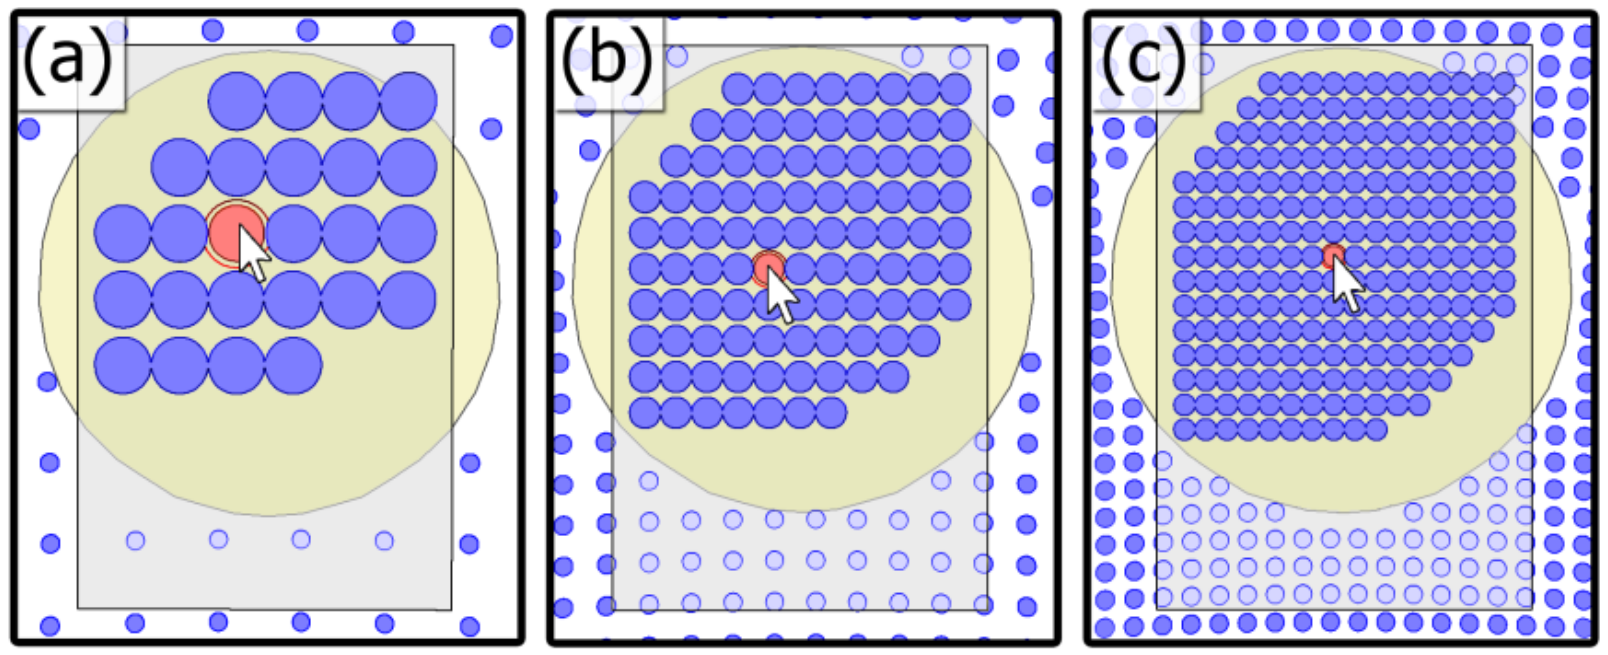
\includegraphics[width=\textwidth]{figures/ch2/dCanvasDensity}
		\caption[\emph{Disambiguation Canvas} --- Densité]{La difficulté de sélection avec le \emph{Disambiguation Canvas} dépend du nombre d'objets présélectionnés dans la première étape. À gauche (a), 25 objets peuvent être sélectionnés, et sont de fait assez gros ; au milieu (b), ils sont 97, et de taille moyenne ; à droite (c) ils sont 224 et nettement plus petits. La loi de Fitts s'applique et nous indique que les cibles seront plus difficiles à sélectionner en environnement dense, du fait de leur taille réduite. Crédit : \cite{debarba2013disambiguation}.}
		\label{fig:dCanvasDensity}
	\end{figure}
	
	\paragraph{Performances}
	Les performances du \emph{Disambiguation Canvas} sont présentées sur la figure~\ref{fig:dCanvasRCPerf}, comparées à celle du \emph{raycasting} classique. Ainsi, l'on constate que cette technique ne fait mieux que le \emph{raycasting} qu'à condition que la densité soit faible ou que les cibles soient petites --- et \emph{a fortiori} les deux à la fois. Ce résultat n'est pas surprenant puisque la sélection en cascade implique nécessairement un coût en divisant la tâche en plusieurs parties, mais ce coût peut rester acceptable si la difficulté de la tâche est suffisamment élevée.
	
	On notera que les taux d'erreurs du \emph{Disambiguation Canvas} sont toujours inférieurs à ceux du \emph{raycasting}, et parfois de beaucoup. C'est une caractéristique courante de la sélection en cascade, qui implique intrinsèquement un biais en faveur de la précision dans le compromis vitesse/précision inhérent à toute tâche de pointage.
	
	\begin{figure}[H]
		\centering
		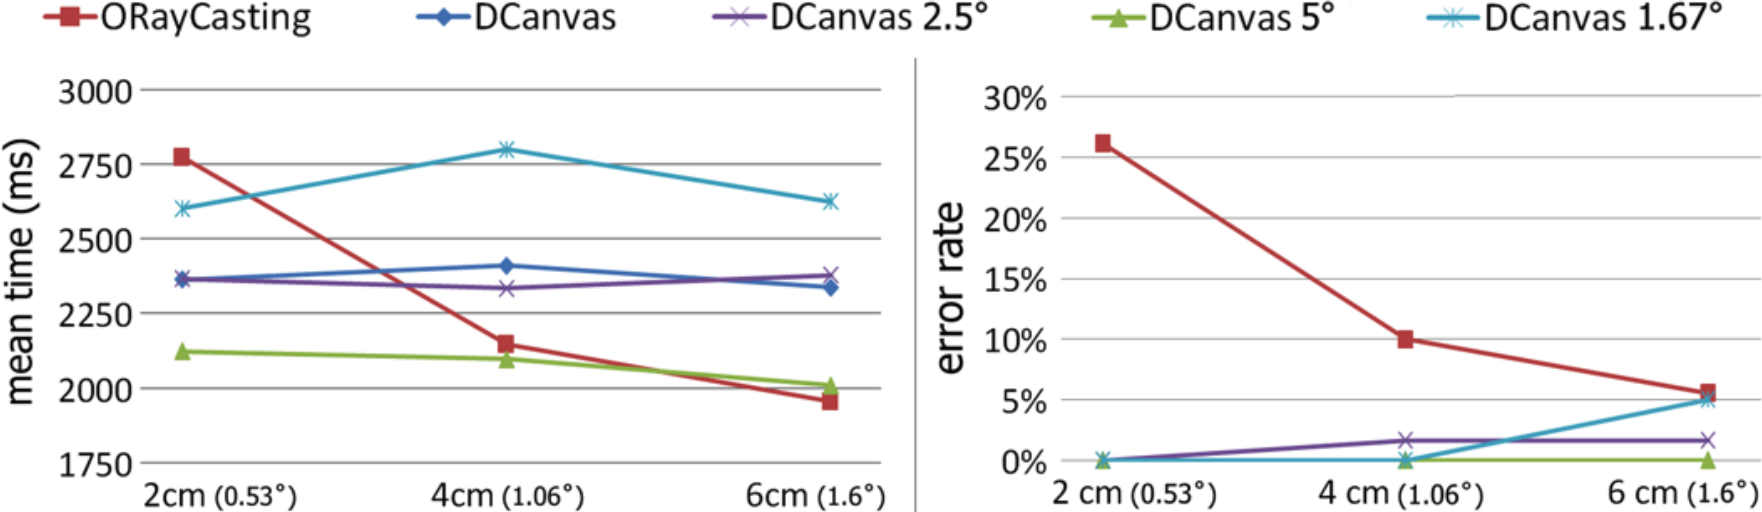
\includegraphics[width=\textwidth]{figures/ch2/dCanvasRCPerf}
		\caption[\emph{Disambiguation Canvas} --- Performances I]{Performances du \emph{Disambiguation Canvas}, comparées à celles du \emph{raycasting} classique, en fonction de la taille des cibles. Pour le \emph{Disambiguation Canvas}, les résultats sont séparés en fonction de la distance angulaire entre les cibles, c'est-à-dire en fonction de leur densité. Plus cette densité est élevée (i.e. plus les angles sont faibles) plus la sélection est difficile car les cibles deviennent petites dans la phase de sélection fine. Les temps de sélection sont affichés sur le graphique de gauche, et les erreurs sur celui de droite. Crédit : \cite{debarba2013disambiguation}.}
		\label{fig:dCanvasRCPerf}
	\end{figure}

	Enfin, précisons que l'agencement calibré des objets décrit sur la figure~\ref{fig:dCanvasLayout} n'était pas utilisé dans cette étude, puisqu'il a été inspiré par les retours des utilisateurs au cours de celle-ci. De fait, on peut supposer avec cette optimisation, les résultats obtenus seraient légèrement meilleurs. Par ailleurs, les utilisateurs rapportent une préférence marquée pour le \emph{Disambiguation Canvas} par rapport au \emph{raycasting}, surtout pour les cibles difficiles, et de même une diminution de la fatigue ressentie.
	
	Pour comparer leur technique à SQUAD, Debarba \emph{et al.} ont légèrement modifié celle-ci en ajoutant après chaque étape « d'affinage » une animation de 200 ms repositionnant les objets dans les quadrants vidés. Quoique cette animation ait un coût, elle permet à l'utilisateur de ne pas perdre la cible qu'il souhaite sélectionner, et donc d'éviter une nouvelle phase de recherche visuelle. Pour des contextes où les objets se ressemblent (voire sont identiques) c'est un compromis qui peut être avantageux (voire indispensable). De plus, l'utilisateur peut déplacer son rayon de sélection pendant l'animation.
	
	Les résultats du \emph{Disambiguation Canvas} comparé à SQUAD sont présentés sur la figure~\ref{fig:dCanvasSPerf}, et sont en faveur de ce premier, sans appel. Plus les objets sont nombreux, plus son avantage croît. On peut toutefois s'interroger sur la solidité de ce résultat avec des objets extrêmement nombreux, puisque la convergence logarithmique de SQUAD permet en principe de gérer un nombre d'objet colossal sans dégradation catastrophique des performances, tandis que le \emph{Disambiguation Canvas} pourrait voir ses performances s'effrondrer lorsque les cibles deviennent trop petites pour être sélectionnées avec une pression du pouce.	
	
	\begin{figure}[H]
		\centering
		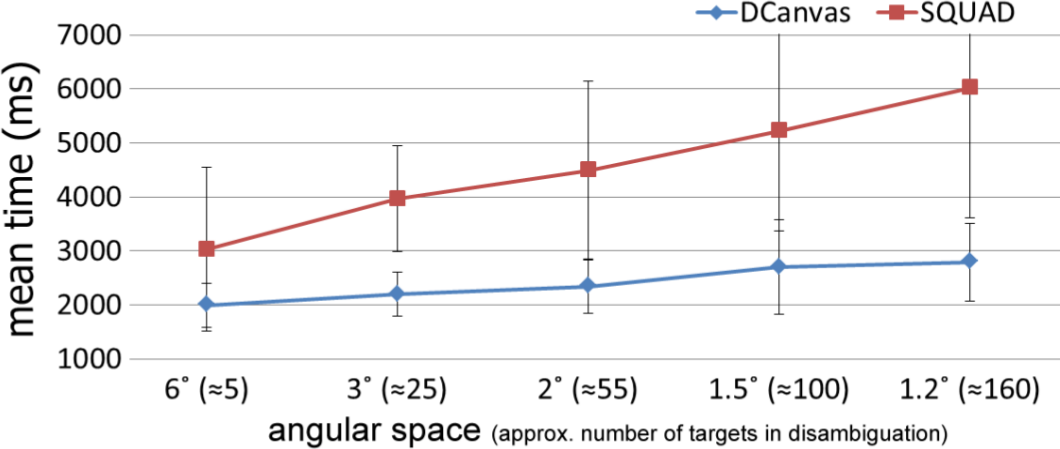
\includegraphics[width=\textwidth]{figures/ch2/dCanvasSPerf}
		\caption[\emph{Disambiguation Canvas} --- Performances II]{Temps de sélection du \emph{Disambiguation Canvas}, comparées à celles de SQUAD, en fonction du nombre de cibles. Les résultats sont clairement en faveur de la première technique sur l'intervalle testé. Crédit : \cite{debarba2013disambiguation}.}
		\label{fig:dCanvasSPerf}
	\end{figure}
	
	Au-delà des temps de sélection, les taux d'erreurs deviendraient certainement problématiques dans ce cas-là, alors qu'ils devraient rester à peu près stables pour SQUAD. Sur l'intervalle de tailles testé, SQUAD a d'ailleurs un léger avantage sur ce plan, avec 0,9~\%{} d'erreurs contre 1,8~\%{} pour le \emph{Disambiguation Canvas}, mais ce dernier résultat reste très bon. Les impressions subjectives des utilisateurs sont grossièrement similaires pour les deux techniques.
		 
	\paragraph{Inconvénients}
	Les choix faits dans la conception du \emph{Disambiguation Canvas} sont différents de ceux de SQUAD, et les évaluations de ces techniques le montrent. Toutefois, les inconvénients majeurs de ces deux techniques sont sensiblement les mêmes, à savoir une perte de contexte en passant d'une phase à l'autre, et de grandes difficultés à reconnaître l'objet à sélectionner s'il est visuellement proche des distracteurs, ou \emph{a fortiori} identique.
	
	Pour pallier ce problème, Debarba \emph{et al.} proposent de gérer la transition entre les deux phases avec une animation permettant de déplacer les objets de l'espace virtuel 3D d'origine vers le rectangle de sélection finale de façon « douce » et progressive, afin que l'utilisateur ne perde pas sa cible des yeux et puisse la retrouver aisément. Dans une certaine mesure, le contexte spatial (local) est préservé, mais il est significativement déformé en règle générale. Cette solution, que les auteurs ont mise en \oe{}uvre mais pas encore évaluée, est illustrée par la figure~\ref{fig:dCanvasContext}.
	
	\begin{figure}[H]
		\centering
		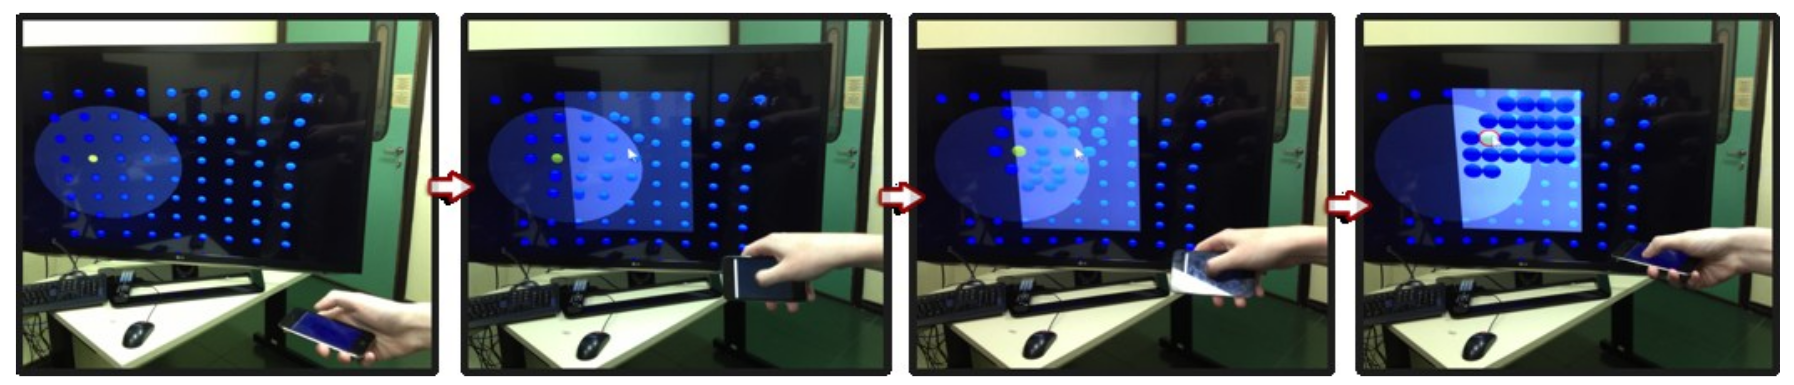
\includegraphics[width=\textwidth]{figures/ch2/dCanvasContext}
		\caption[\emph{Disambiguation Canvas} --- Animation de transition]{Animation pendant la transition entre la phase de présélection du \emph{Disambiguation Canvas} et la phase de disambiguïsation. Les objets sont réarrangés « en douceur » ce qui permet à l'utilisateur de suivre la cible des yeux afin de ne pas la perdre, et de préserver, dans une certaine mesure, le contexte spatial. Crédit : \cite{debarba2013disambiguation}.}
		\label{fig:dCanvasContext}
	\end{figure}
	
	Bien que ce palliatif puisse améliorer les performances de sélection quand les objets se ressemble, on peut douter de son efficacité quand ils sont identiques. De plus, le contexte spatial demeure très dégradé en passant d'une phase à l'autre, et les cibles ne sont, là encore, que statiques. Il apparaît donc difficile d'appliquer le \emph{Disambiguation Canvas} à des contextes caractérisés par des objets semblables, nombreux et mobiles.
	
	\subsubsection{Inconvénients généraux}
	Les techniques de sélection en cascade pouvant prendre des formes très diverses, leurs avantages et inconvénients sont également divers. Néanmoins, elles ont pour principe commun de travailler successivement à différentes échelles, ce qui peut être perturbant en environnement immersif, particulièrement lorsque l'on cherche à maintenir une correspondance entre l'espace moteur et l'espace virtuel. Néanmoins, si les gains de performances offerts par la sélection en cascade sont importants, cette perturbation pourrait être une contrepartie acceptable.
	
	Notons que la phase grossière ne se fait pas nécessairement avec le même périphérique que la phase fine ; elle peut par exemple se baser sur une estimation de la direction du regard de l'utilisateur, voire se faire automatiquement, par exemple lorsque l'utilisateur focalise son regard sur une zone approximativement constante pendant un certain laps de temps.
	
	En revanche, on retrouve couramment avec les techniques de sélection en cascade une dégradation, voire une perte du contexte spatial lorsque l'on passe de la phase grossière à la phase fine~\cite{kopper2011rapid, debarba2013disambiguation}. C'est potentiellement plus problématique que la perte de correspondance entre l'espace moteur et l'espace virtuel, et d'autant plus gênant que la phase fine est généralement peu adaptée à des cibles mobiles, qui nous intéressent particulièrement dans ces travaux.
	
	Cela ne revient pas à rejeter le principe de la sélection en cascade pour les applications qui nous intéressent, mais à souligner que les solutions existantes sont généralement peu adaptées à de telles tâches, et qu'une technique de sélection en cascade appropriée nécessiterait probablement d'être pensée pour les cibles mobiles dès le départ.


% 40% to 70% of gaze displacement is provided by head rotation, while the remaining 60% to 30% result from angular displacement of the eyes in orbit
% http://books.google.fr/books?id=h9FEnj3C7MoC&pg=PA102&lpg=PA102&dq=head+tracking+70%25+of+gaze&source=bl&ots=cp8OJm_G-1&sig=0jsxP3V20VGuxmIvg9CB1sUcyeU&hl=en&sa=X&ei=JFUsU-rVJYam0AW1zYDwAw&redir_esc=y#v=onepage&q&f=false
\section{Suivi de la tête et des yeux}
	\subsection{Principe général et avantages}
	Une estimation de la direction du regard de l'utilisateur peut être utilisée soit pour sélectionner directement la cible (ce qui peut nécessiter beaucoup de précision, quand la cible est petite) soit pour sélectionner une zone d'intérêt, dans la phase grossière d'une sélection en cascade. Il y a au moins deux façons d'estimer la direction du regard : la première consiste à capturer les mouvements de la tête de l'utilisateur, et à supposer qu'il regarde droit devant lui. Comme cette hypothèse est généralement fausse, on génère un cone dont le sommet est la tête de l'utilisateur, et dont l'axe de révolution correspond à la direction (estimée) du regard. Or, 40~\%{} à 70~\%{} du déplacement du regard est déterminé par la rotation de la tête, tandis que le reste résulte des mouvements oculaires.[ref bouquin] Si cela s'avère souvent insuffisant pour effectuer une sélection directe, le suivi de tête peut présenter un certain intérêt pour la sélection en cascade.
		
	Pour estimer la direction du regard avec plus de précision, on peut capturer non seulement la position et l'orientation de la tête, mais également l'orientation des yeux. Cette option séduisante présente toutefois quelques difficultés :
	\begin{itemize}
		\item Les performances dépendent de la couleur des yeux ;[ref]
		\item Le suivi des yeux ne fonctionne pas toujours bien en environnement sombre, par exemple dans un CAVE ;[ref]
		\item Les lunettes stéréoscopiques occultent partiellement les yeux pour les \emph{trackers} oculaires, et réduisent la luminosité du blanc des yeux ;[ref]
		\item Le suivi des yeux, souvent combiné à celui de la tête, est plus coûteux que celui de la tête seule ;
		\item Le fait d'utiliser ses yeux pour sélectionner un objet fait du regard une action, rend les utilisateurs conscients de la direction dans laquelle ils regardent, ce qui peut être troublant.
	\end{itemize}

	Par conséquent, l'utilisation de suivi des yeux se montre souvent difficile à mettre en œuvre, quoique les progrès techniques puissent, dans un futur proche, pallier au moins partiellement ces difficultés.
	
	\subsection{\emph{Look and Touch}}
	\subsubsection{Principe et avantages}
	~\cite{stellmach2012look}
	
	\subsubsection{Inconvénients}
	
	\subsection{Inconvénients généraux}
	
\section{\emph{Kinematic Endpoint Prediction}}
	\subsection{Principe et avantages}
	\cite{lank2007endpoint}
	\subsection{Inconvénients}
		
\section{\emph{Speed}}
	\subsection{Principe et avantages}
	\emph{Speed}~\cite{wonner2011speed} est une heuristique de prédiction de cible. Quand l'utilisateur tente de sélectionner une cible, il déplace son curseur vers elle d'une façon que l'on peut séparer en deux phases. Au cours de la première phase, il accélère, tandis qu'il décélère pendant la seconde. C'est dans cette dernière que l'utilisateur est généralement le plus précis. \emph{Speed} base donc sa prédiction de cible sur la phase de décélération. L'heuristique estime la distance que le curseur finira par couvrir à partir de la vitesse du curseur, par ajustement de courbe avec celle d'une fonction quadratique. Quand le curseur a parcouru 85~\%{} de la distance totale estimée, \emph{Speed} utilise la position et la direction courantes du curseur, ainsi que l'estimation de la distance qu'il lui reste à parcourir pour prédire sa destination finale, et par conséquent, la cible visée par l'utilisateur. Cette technique fournit de meilleurs résultats que les précédentes approches de ce type qui ne faisaient pas de distinction entre les phase d'accélération et de décélération.[ref]
			
	\subsection{Inconvénients}
	Cependant, \emph{Speed} part du principe qu'au moment où l'utilisateur décide de sélectionner une cible et commence à déplacer le curseur, il sait quelle cible il veut choisir, où elle se trouve, et donc où placer son curseur. De fait, le mouvement effectué est approximativement rectiligne. Mais si les cibles sont mobiles, alors la trajectoire du curseur ne peut plus être supposée rectiligne. Par conséquent, la précision de \emph{Speed} avec des cibles mobiles est sujette à caution. C'est d'autant plus vrai en environnement dense, car une petite erreur de prédiction a d'autant plus de chances d'aboutir à la sélection d'un distracteur que ceux-ci sont nombreux et près de la cible visée.


\section{\emph{Intenselect}}
	\subsection{Principe et avantages}
	~\cite{de2005intenselect}
	
	\subsection{Inconvénients}
		
\section{Hook}
	\subsection{Principe et avantages}
	\emph{Hook} est une heuristique de prédiction de cible. Elle se base sur une évaluation continue de la distance entre le curseur et les cibles potentielles. Celles-ci sont triées par ordre de proximité, et les $NCT$ (\emph{Number of Closest Targets} cibles les plus proches du curseur voient leur score augmenter à chaque boucle de l'heuristique, et augmenter d'autant plus fortement qu'elles sont proches du curseur. Toutes les autres cibles voient leur score diminuer, et diminuer d'autant plus fortement qu'elles sont éloignées du curseur.
		
	La cible potentielle dont le score est le plus élevé est considérée comme celle que l'utilisateur cherche probablement à sélectionner. La sélection peut donc se faire par simple pression d'un bouton, sans contrainte particulière sur la position du curseur au moment où elle est déclenchée.
		
	\emph{Hook} présente plusieurs avantages. Cette technique spécifiquement conçue pour les cibles mobiles fonctionne également pour les cibles statiques. Elle n'ajoute aucun encombrement visuel, ne transforme pas le curseur, ne modifie pas l'apparence des cibles, et n'interrompt pas l'animation ou la simulation en cours. L'évaluation menée par Michael Ortega montre que \emph{Hook} est non seulement plus rapide que le \emph{Bubble Cursor} en 2D comme en 3D, mais permet en plus des taux d'erreur plus faibles. Lorsque les cibles sont rapides, le taux d'erreur peut être moindre d'un facteur supérieur à 4~\cite{ortega2013hook}.
	
	\subsection{Inconvénients}

\clearpage
